% !TeX root = ./ms.tex
\documentclass[modern]{aastex62}

% Load the corTeX style definitions
% !TeX root = ./ms.tex
% All the packages
\usepackage{url}
\usepackage{amsmath}
\usepackage{mathtools}
\usepackage{amssymb}
\usepackage{natbib}
\usepackage{graphicx}
\usepackage{calc}
\usepackage{etoolbox}
\usepackage{xspace}
\usepackage[T1]{fontenc} % https://tex.stackexchange.com/a/166791
\usepackage{textcomp}
\usepackage{ifxetex}
\ifxetex
  \usepackage{fontspec}
  \defaultfontfeatures{Extension = .otf}
\fi
\usepackage{fontawesome}
\usepackage{listings}
\usepackage{nicefrac}
\usepackage[bb=boondox]{mathalfa}
\usepackage{booktabs}
\usepackage{longtable}

% Shorthand for this paper
\newcommand{\starry}{\textsf{starry}\xspace}
\newcommand{\Python}{\textsf{Python}\xspace}
\newcommand{\cpp}{\textsf{C}++\xspace}
\newcommand{\bvec}[1]{{\ensuremath{\mathbf{#1}}}}
\newcommand{\xxx}[1]{{\color{red}#1}}
\DeclarePairedDelimiter\floor{\lfloor}{\rfloor}
\DeclarePairedDelimiter\ceil{\lceil}{\rceil}
\newcommand{\imag}{{\ensuremath{\mathbb{i}}}}
\newcommand{\quadquad}{\quad\quad\quad\quad}

\newcommand{\R}{\bvec{R}}
\newcommand{\AOne}{\bvec{A_1}}
\newcommand{\alm}{\bvec{a}}
\newcommand{\x}{\bvec{x}}
\newcommand{\D}{D}
\newcommand{\Doppler}{\bvec{D}}
\newcommand{\Surf}{\mathcal{S}}
\newcommand{\Curve}{\mathcal{C}}
\newcommand{\Dargs}{\bvec{d}}
\newcommand{\lmax}{\ensuremath{l_\mathrm{max}}}
\newcommand{\spot}{\texttt{SPOT}\xspace}
\newcommand{\vogtstar}{\texttt{VOGTSTAR}\xspace}
\newcommand{\kT}{\boldsymbol{\kappa}^\top}
\newcommand{\rhoT}{\boldsymbol{\rho}^\top}
\newcommand{\ylmbasis}{\boldsymbol{\psi}^\top}
\newcommand{\pbasis}{\boldsymbol{\phi}^\top}
\newcommand{\pbasisn}{\ensuremath{\phi_n}}
\newcommand{\azero}{\ensuremath{\bvec{a_0}}}

% References to text content
\newcommand{\documentname}{\textsl{article}}
\newcommand{\figureref}[1]{\ref{fig:#1}}
\newcommand{\Figure}[1]{Figure~\figureref{#1}}
\newcommand{\figurelabel}[1]{\label{fig:#1}}
\renewcommand{\eqref}[1]{\ref{eq:#1}}
\newcommand{\Eq}[1]{Equation~(\eqref{#1})}
\newcommand{\eq}[1]{\Eq{#1}}
\newcommand{\eqalt}[1]{Equation~\eqref{#1}}

% Add code, proof, and animation hyperlinks
\definecolor{linkcolor}{rgb}{0.1216,0.4667,0.7059}
\newcommand{\codeicon}{{\color{linkcolor}\faFileCodeO}}
\newcommand{\prooficon}{{\color{linkcolor}\faPencilSquareO}}
\newcommand{\codelink}[1]{\href{https://github.com/user/repo/blob/fe12fa16a5cc76c1ba72d97241fb9545da144edf/tex/figures/#1.py}{\codeicon}\,\,}
\newcommand{\animlink}[1]{\href{https://github.com/user/repo/blob/fe12fa16a5cc76c1ba72d97241fb9545da144edf/tex/figures/#1.gif}{\animicon}\,\,}
\newcommand{\prooflink}[1]{\href{https://github.com/user/repo/blob/fe12fa16a5cc76c1ba72d97241fb9545da144edf/tex/proofs/#1.ipynb}{\raisebox{-0.1em}{\prooficon}}}
\newcommand{\cilink}[1]{\href{https://dev.azure.com/user/repo/_build}{#1}}


% Define a proof environment for open source equation proofs
\newtagform{eqtag}[]{(}{)}
\newcommand{\currentlabel}{None}
\newenvironment{proof}[1]{%
  \ifstrempty{#1}{%
    \renewtagform{eqtag}[]{\raisebox{-0.1em}{{\color{red}\faPencilSquareO}}\,(}{)}%
  }{%
    \renewtagform{eqtag}[]{\prooflink{#1}\,(}{)}%
  }%
  \usetagform{eqtag}%
  \renewcommand{\currentlabel}{#1}
  \align%
}{%
  \endalign%
  \renewtagform{eqtag}[]{(}{)}%
  \usetagform{eqtag}%
  \message{<<<\currentlabel: \theequation>>>}%
}

% Display the runtime on Azure
\usepackage[skins]{tcolorbox}
\newtcbox{\figtimebox}{enhanced,nobeforeafter,tcbox raise=-0.8mm,boxrule=0.6pt,
  top=0.5mm,bottom=0mm,right=0mm,left=6mm,arc=1pt,boxsep=2pt,
  before upper={\vphantom{dlg}},colframe=linkcolor,coltext=linkcolor,
  fontupper=\sffamily\bfseries\tiny,colback=white,overlay={\begin{tcbclipinterior}
        \fill[linkcolor] (frame.south west)
        rectangle node[text=white,font=\sffamily\bfseries\tiny,rotate=0]{CPU}
        ([xshift=6mm]frame.north west);\end{tcbclipinterior}}}
\robustify{\figtimebox}
\pdfstringdefDisableCommands{%
  \def\figtimebox#1{'#1'}%
}
\newcommand{\figtime}[1]{\IfFileExists{figures/#1.py.time}%
  {%
    \cilink{\figtimebox{\input{figures/#1.py.time}\unskip s}}
  }{}}

% Define the `oscaption` command for open source figure captions
\newcommand{\oscaption}[2]{\caption{#2 \codelink{#1} \figtime{#1}}}

% Code examples
\definecolor{codegreen}{rgb}{0,0.6,0}
\definecolor{codegray}{rgb}{0.5,0.5,0.5}
\definecolor{codepurple}{rgb}{0.58,0,0.82}
\definecolor{backcolour}{rgb}{0.95,0.95,0.95}
\lstdefinestyle{mystyle}{
  backgroundcolor=\color{backcolour},
  commentstyle=\color{codegreen},
  keywordstyle=\color{magenta},
  numberstyle=\tiny\color{codegray},
  stringstyle=\color{codepurple},
  basicstyle=\small\ttfamily,
  breakatwhitespace=false,
  breaklines=true,
  captionpos=b,
  keepspaces=true,
  numbers=left,
  numbersep=5pt,
  showspaces=false,
  showstringspaces=false,
  showtabs=false,
  tabsize=2,
  aboveskip=1em,
  belowskip=1em,
  keywords=[2]{map},
  keywordstyle=[2]{\color{black!80!black}},
  upquote=true
}
\lstset{style=mystyle}

% Typography obsessions
\setlength{\parindent}{3.0ex}
\renewcommand\quad{\hskip\fontdimen3\font}

% https://tex.stackexchange.com/a/184474
\usepackage{stackengine,scalerel}
\def\lnlam{\ThisStyle{\ensurestackMath{\stackon[-2.4\LMpt]{%
        \SavedStyle\lambda}{\kern-.5pt\kern\LMpt\rule{1\LMex}{.25pt+.15\LMpt}}}}}

% Load custom style
% Packages
\usepackage{amsmath}
\usepackage{fontspec}
\usepackage{unicode-math}
\usepackage{xifthen}
\usepackage{stackengine}

% Integrals
\newcommand{\vint}[2]{\int\limits_{#1}#2\dd\varphi}
\newcommand{\dd}{\ensuremath{\text{d}}}

% Special functions
\newcommand{\sgn}{{\text{sgn}}}
\newcommand{\atantwo}{{\text{arctan2}}}

% Misc. macros
\newcommand{\STARRYQUADPOINTS}{100\xspace}

% Basis vectors
\newcommand{\bg}{\ensuremath{\tilde{\mathbf{g}}}}
\newcommand{\bp}{\ensuremath{\tilde{\mathbf{p}}}}
\newcommand{\by}{\ensuremath{\tilde{\mathbf{y}}}}

% Cartesian unit vectors
\newcommand{\xhat}{\ensuremath{\pmb{\hat{x}}}\xspace}
\newcommand{\yhat}{\ensuremath{\pmb{\hat{y}}}\xspace}
\newcommand{\zhat}{\ensuremath{\pmb{\hat{z}}}\xspace}

% Primitive integrals
\newcommand{\sTe}{\ensuremath{\mathbf{s}^\top}}
\newcommand{\rTe}{\ensuremath{\mathbf{r}^\top}}
\newcommand{\sT}{\ensuremath{\mathbbb{s}^\top}}
\newcommand{\rT}{\ensuremath{\mathbbb{r}^\top}}
\newcommand{\pT}{\ensuremath{\mathbbb{p}^\top}}
\newcommand{\tT}{\ensuremath{\mathbbb{t}^\top}}
\newcommand{\qT}{\ensuremath{\mathbbb{q}^\top}}

% Helper integrals
\newcommand{\iI}{\ensuremath{\mathbb{i}}}
\newcommand{\iJ}{\ensuremath{\mathbb{j}}}
\newcommand{\iU}{\ensuremath{\mathbb{u}}}
\newcommand{\iW}{\ensuremath{\mathbb{w}}}
\newcommand{\viI}{\ensuremath{\mathbbb{i}}}
\newcommand{\viJ}{\ensuremath{\mathbbb{j}}}
\newcommand{\viU}{\ensuremath{\mathbbb{u}}}
\newcommand{\viW}{\ensuremath{\mathbbb{w}}}

% Elliptic integrals
\newcommand{\DE}{\Delta \mathbf{E}(k^2, \vkappa)}
\newcommand{\DF}{\Delta \mathbf{F}(k^2, \vkappa)}

% Angles
\newcommand{\vkappa}{\pmb{\kappa}}
\newcommand{\vlambda}{\pmb{\lambda}}
\newcommand{\vxi}{\pmb{\xi}}
\newcommand{\coshalfkap}[1][]{%
    \ifthenelse{%
        \equal{#1}{}
    }{
        \cos\left(\frac{\vkappa}{2}\right)
    }{
        \cos^{#1}\left(\frac{\vkappa}{2}\right)
    }}
\newcommand{\sinhalfkap}[1][]{%
    \ifthenelse{%
        \equal{#1}{}
    }{
        \sin\left(\frac{\vkappa}{2}\right)
    }{
        \sin^{#1}\left(\frac{\vkappa}{2}\right)
    }}

% Other
\newcommand{\vmax}{{v_\text{max}}}

% Bibliography
\bibliographystyle{aasjournal}

% Begin!
\begin{document}

% Title
\title{Analytic Occultation Light Curves in Reflected Light}

% Author list
\author[0000-0002-0296-3826]{Rodrigo Luger}
\email{rluger@flatironinstitute.org}
\affil{Center~for~Computational~Astrophysics, Flatiron~Institute, New~York, NY}
%

\begin{abstract}
    Abstract here.
    %
    \href{https://github.com/rodluger/starrynight}{\color{linkcolor}\faGithub}
\end{abstract}

%
\section{Introduction}
\label{sec:intro}
%
\xxx{A few paragraphs of introduction here. \citet{Russell1906}.}

Our goal in this paper is to derive analytic expressions for the
flux received by a distant observer from a non-uniform Lambert sphere
illuminated by a monochromatic source that may or may not be
occulted by a (possibly different) spherical body. This applies, for example,
to the
case of exoplanet phase curves, exoplanet secondary
eclipse (occultation) light curves, or exoplanet-moon and exoplanet-exoplanet
occultations, all seen in reflected light. We explicitly assume the reflecting
body is Lambertian, i.e., it scatters light isotropically, although with an
intensity that varies across the surface according to a spatially-dependent
albedo $A$. Throughout this paper, we will take $A$ to mean the \emph{spherical}
albedo, the fraction of power incident on a body at a given wavelength
that is scattered back out to space (in all directions).
Note that the spherical albedo
is closely related to the Bond albedo: the Bond albedo is the stellar
flux-weighted integral of $A(\lambda)$ over all wavelengths $\lambda$
\citep[see, e.g.,][]{Seager2010}.

As in \citet{Luger2019}, we compute fluxes by first expanding the surface
in terms of spherical harmonics.
While in \citet{Luger2019} we expanded the emissivity of the surface, here
we instead expand the spherical albedo $A$.
Specifically, if $\bvec{y}$ is the vector
of spherical harmonic coefficients describing the albedo anywhere on
the surface and
$\by$ is the spherical harmonics basis (Equation~\ref{eq:by}),
the albedo $A$ at a point $(x, y)$ on the sky-projected disk of the body
is given by the dot product
%
\begin{align}
    \label{eq:albedo}
    A(x, y) = \by^\top (x, y) \, \bvec{y}
    \quad.
\end{align}
%
The flux measured from this body is the surface integral over the visible
portion of the body's projected disk of the albedo $A$
times the illumination profile $\mathcal{I}$ of the surface, given by
Lambert's law as
%
\begin{align}
    \label{eq:LambertsLaw}
    \mathcal{I}(\phi) = \mathcal{I}_0 \, \text{max}\big( 0, \cos\phi \big)
    \quad,
\end{align}
%
where $\mathcal{I}_0$ is the peak illumination (at the sub-source point).
%

The piecewise nature of the illumination function at the day/night terminator
makes the problem of computing the visible flux particularly difficult; most
studies to date have tackled the problem numerically, by discretizing the surface
and computing the relevant integrals by summing over the visible
pixels \xxx{(cite)}. Recently, \citet{Haggard2018} developed an analytic
framework for computing light curves of unocculted bodies illuminated
by a point source. In this paper, we re-derive their solution under the
\starry framework and extend it for the first time to the case where
the body is occulted by another spherical body, which may or may not be the
illumination source.

In \citet{Luger2019}, we reduced the problem of computing the flux from
an occulted body in thermal (emitted) light to a series of efficient, analytical
operations involving trigonometric functions of the position and size of the
occultor and certain complete elliptic integrals. In the case of reflected
light, however, the change in the limits of integration due to the
unilluminated night side breaks many of the symmetries that simplified
the flux calculation. In particular, the limits of integration now depend
on the solution to a quartic equation specifying the points of intersection
between the occultor and the day/night terminator, and the solution to
those integrals is now a function of \emph{incomplete} elliptic integrals.
The procedure for computing the flux is therefore significantly more complex.
%
We therefore defer all calculations to the Appendix, and devote the body of
the paper to validating and demonstrating applications of our approach.

\section{Reflected light curves in \starry}
\label{sec:validation}

\subsection{Sample light curves}
\label{sec:sample}

\begin{figure}[t!]
    \begin{centering}
        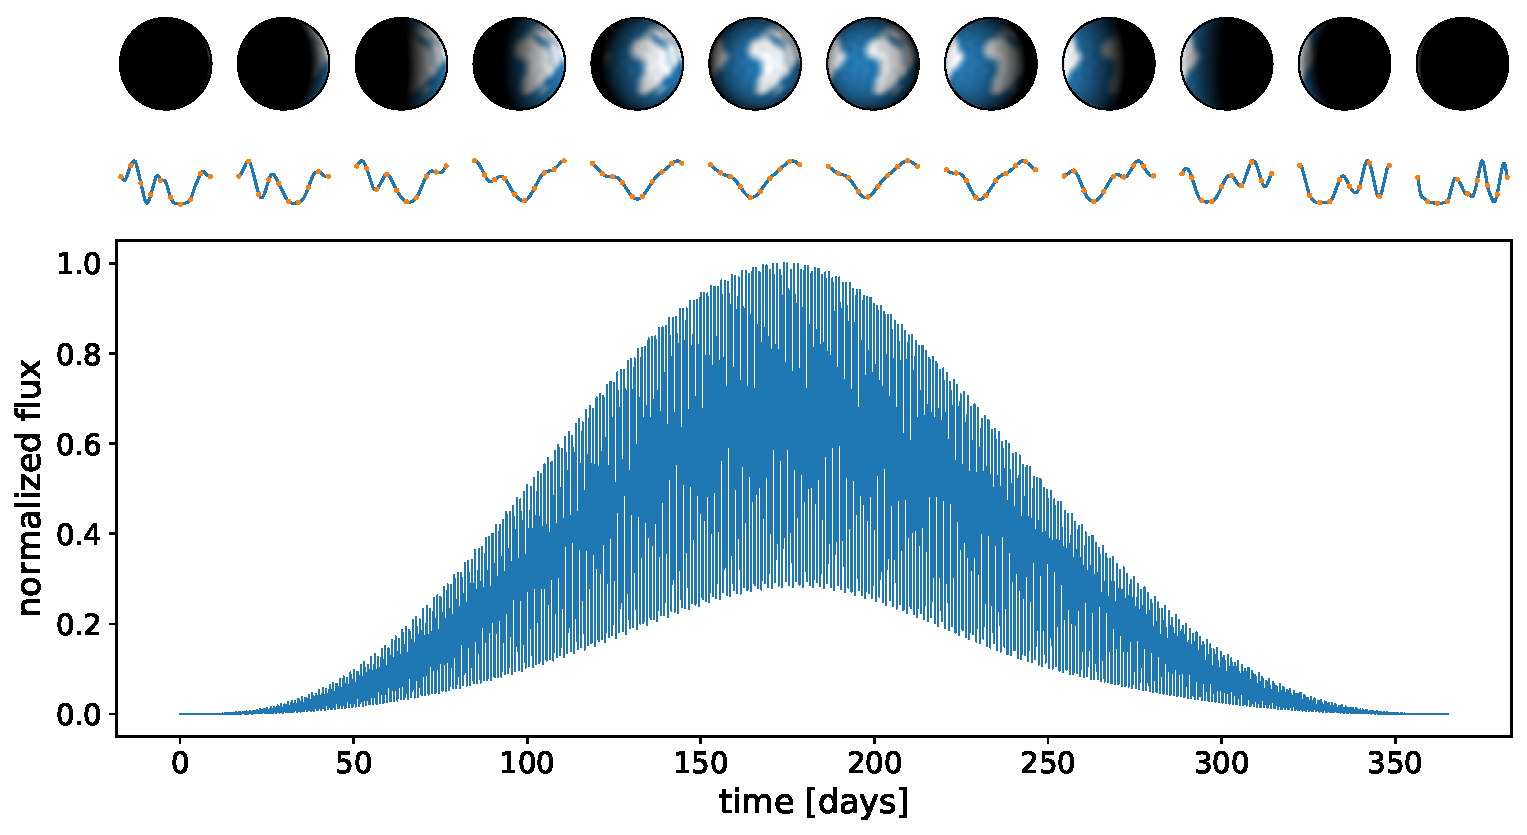
\includegraphics[width=\linewidth]{figures/earthphase.pdf}
        \oscaption{earthphase}{%
            Mock reflected light phase curve of the cloudless Earth expanded
            to spherical harmonic degree $l = 25$, viewed along the
            ecliptic. The main plot shows the phase curve over the course of
            one year.
            The images at the top show the corresponding progression of
            the phases of the Earth, from new phase to full phase and back
            to new phase. Below each image we show a normalized 24-hour
            segment of the light curve at that phase (blue).
            Orange dots correspond
            to the flux computed from brute force numerical integration on
            a grid of
            ${\sim}10^6$ points.
            \label{fig:earthphase}
        }
    \end{centering}
\end{figure}

Figure~\ref{fig:earthphase} shows a sample application of the algorithm
developed in this paper: a reflected light phase curve of the
Earth over the course of one year. The model is computed using the
methodology in Appendix~\ref{sec:solution-no-occ} from an $l=25$
spherical harmonic expansion of the cloudless Earth, where the oceans
are given an albedo of zero and the continents an albedo of unity
(note, however, that since the light curve is normalized, the model does
not depend on the value of the latter).
The Earth is assumed to be a perfect Lambertian scatterer,
so effects like the phase dependence of Rayleigh scattering and
specular reflection (glint) from the oceans are neglected
(but see \S\ref{sec:extensions} for an extension of the model to
non-Lambertian scatterers).
The observer is assumed to be along
the ecliptic, so the illumination source is along the $x-z$ plane of a
right-handed Cartesian coordinate system, with $\hat{z}$ pointing toward the
observer and $\hat{x}$ pointing to the right on the sky. The axis of rotation
of the Earth is therefore tilted clockwise away from
$\hat{y}$ by $23.5^\circ$.
The images at the top show snapshots of the disk of the Earth throughout
the observation; below each one, we plot in blue the normalized phase curve
at that phase over a single rotation. The orange dots correspond to a
brute force numerical solution, obtained by discretizing the disk
on a grid of ${\sim}10^6$ points and summing over the dayside.
The models agree to within the
numerical precision of the brute force solution (about 100 ppm of the
planetary flux in this case).

While the dominant signal in the phase curve is the sine-like envelope
due to the changing phases of the Earth, the local behavior of the light
curve at each phase is complex and varies significantly over the course
of the year. Unlike phase curves in thermal light, which primarily encode
low-order spatial information (since the region of integration is always
the full disk), phase curves in reflected light encode information at
different scales depending on the phase. At crescent phase, the region of the
disk contributing to the total flux is a narrow lune; these measurements
therefore encode information primarily about high-$l$ modes. At full
phase, the region of integration is the full disk, so these measurements
encode information about low-$l$ modes. Furthermore, because of the obliquity
of the Earth,
the orientation of the crescent lune changes relative to features on the
surface over the course of one orbit, changing the relative contribution of
different portions of the surface to the flux and increasing the
overall information content of the observation.
As we will show in \S\ref{sec:information}, the information content of
reflected light phase curves is overwhelmingly higher than that of
phase curves in thermal light, particularly for planets with significant
obliquity.

%

\begin{figure}[t!]
    \begin{centering}
        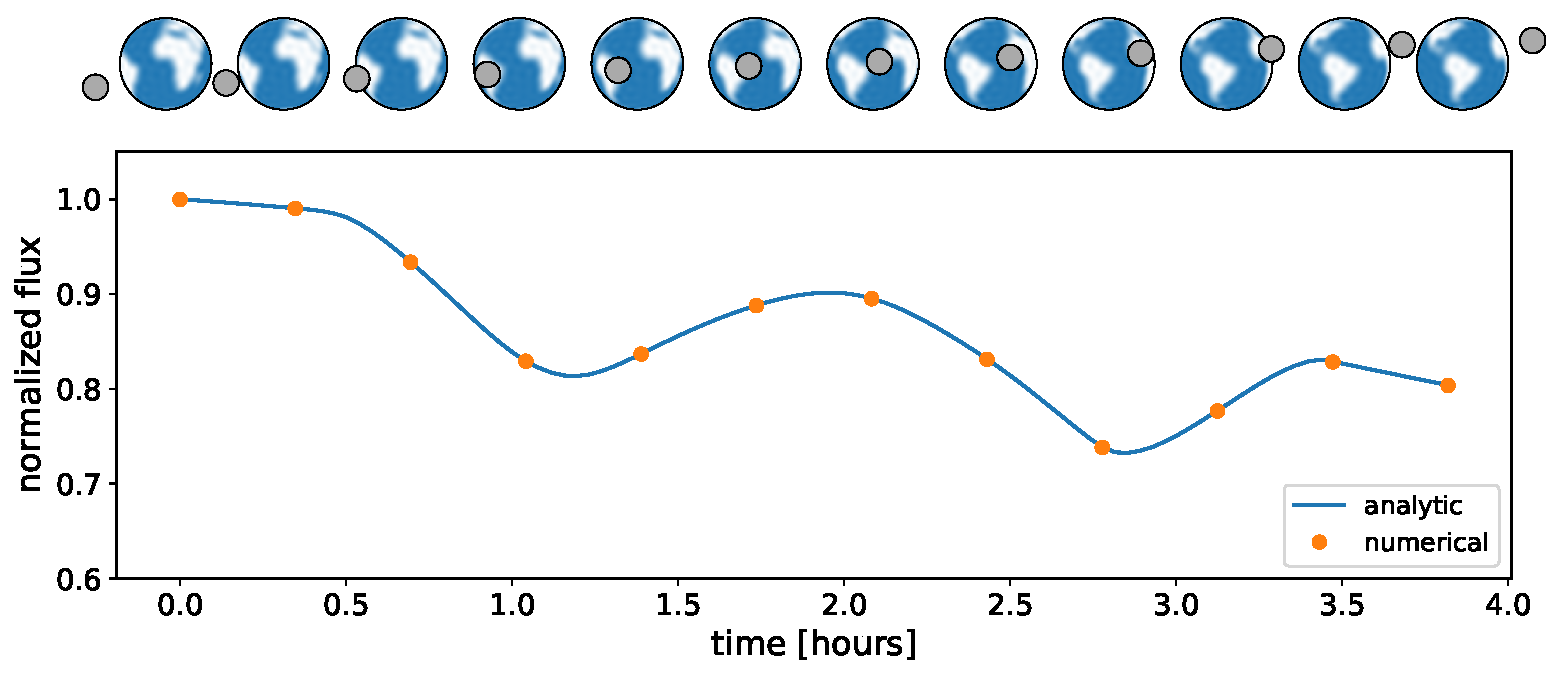
\includegraphics[width=\linewidth]{figures/earthmoon_emitted.pdf}
        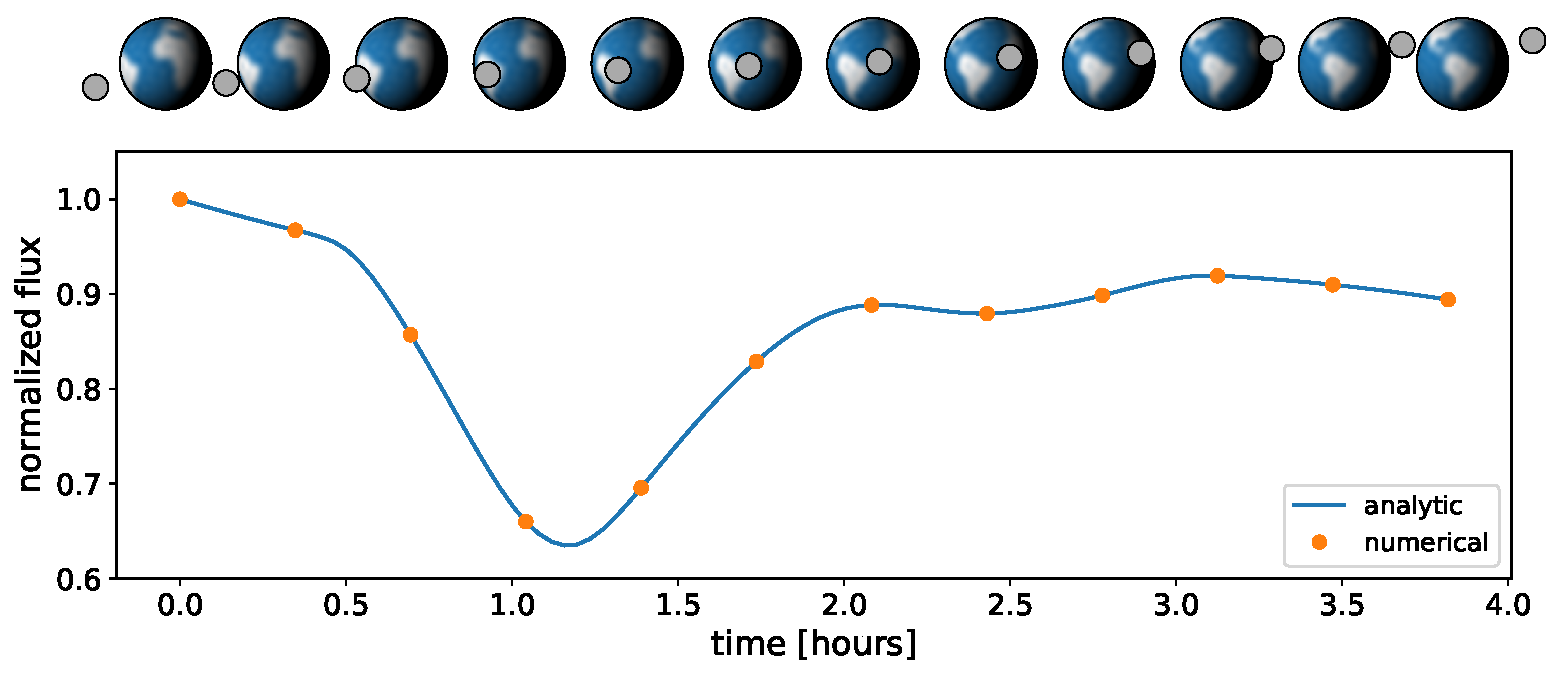
\includegraphics[width=\linewidth]{figures/earthmoon.pdf}
        \oscaption{earthmoon}{%
            Mock light curves of the Moon occulting a rotating,
            cloudless Earth expanded to spherical harmonic degree $l = 25$.
            Black curves show the analytic solution; orange dots correspond
            to brute force numerical integration on a grid of
            ${\sim}10^6$ points.
            The top panel shows the light curve in emitted light and is
            the same as in Figure~7 in \citet{Luger2019}.
            The bottom panel (this work) shows the same light curve in
            reflected light during northern summer.
            \label{fig:earthmoon}
        }
    \end{centering}
\end{figure}

Figure~\ref{fig:earthmoon} shows another light curve of the rotating
Earth, but this time taken during an occultation by the Moon. The map
of the Earth is the same as before, but the observer is now in the
equatorial frame of the Earth.
The top panel is a reproduction of
Figure~7 in \citet{Luger2019} for the case of thermal light,
where the Moon is seen to travel across the
disk of the Earth from southwest to northeast, progressively occulting
South America (dip), the Atlantic (peak), and Africa (dip).
As before,
the blue curve is the analytic solution and the orange dots correspond
to the numerical solution.

The bottom panel of the figure shows a light curve for the
same occultation geometry, but seen instead in reflected light, with the
Sun to the top left and slightly out of the page, corresponding to
some point during northern summer. Note the same dip-peak-dip pattern,
albeit with significantly different amplitudes. In particular, the
transit across South America is deeper, since it occurs close to local
noon, when the illumination is highest; conversely, the transit across
Africa occurs close to local dusk, when the illumination is close to zero.
As before, the light curves computed using \starry agree to within the
numerical precision of the brute force solution.

%

\begin{figure}[p!]
    \begin{centering}
        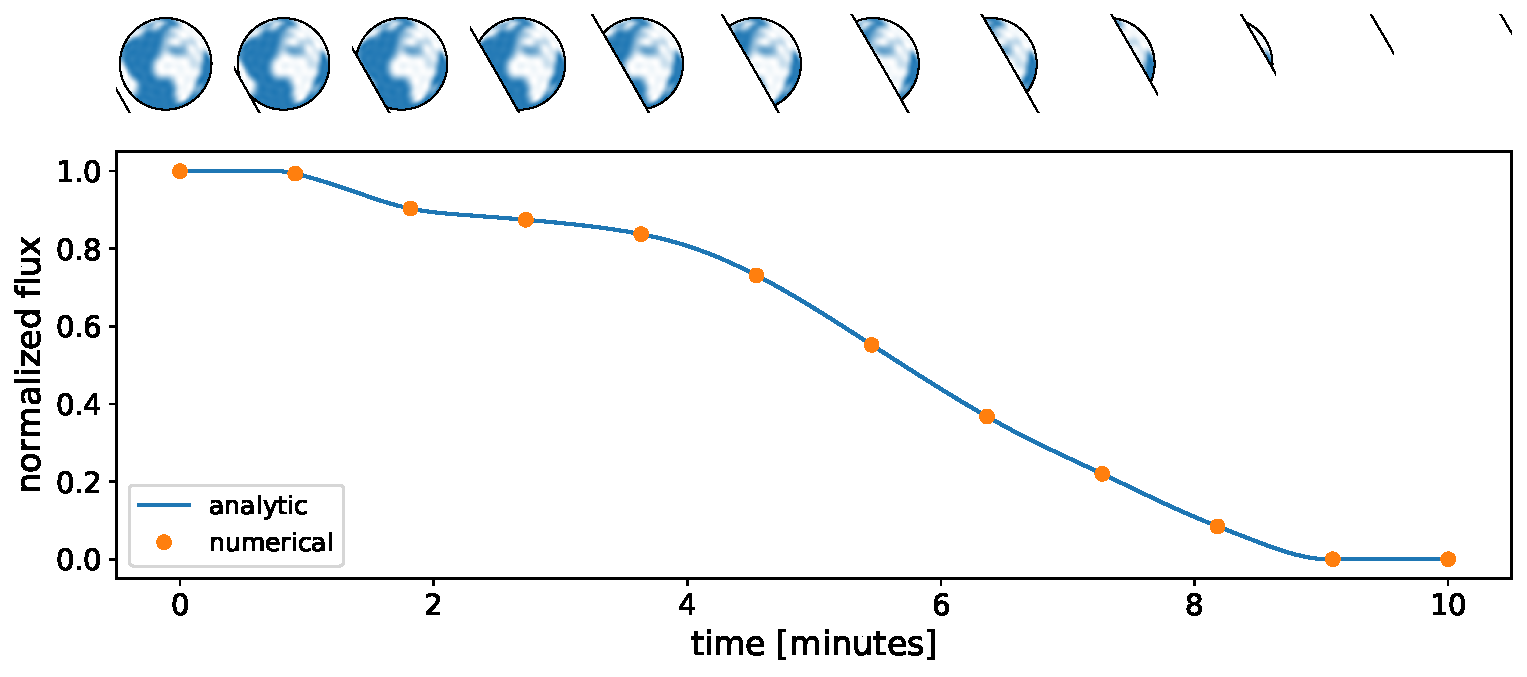
\includegraphics[width=\linewidth]{figures/earthsun_emitted.pdf}
        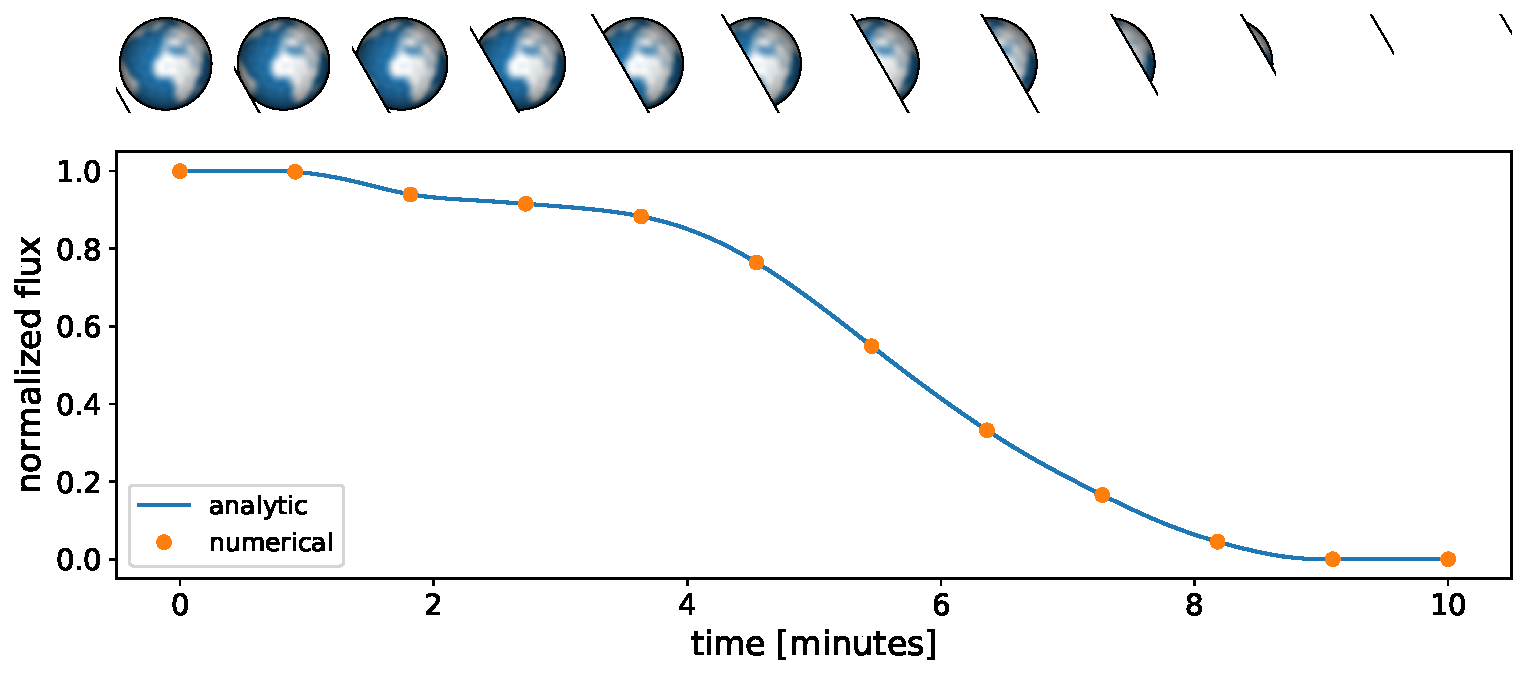
\includegraphics[width=\linewidth]{figures/earthsun.pdf}
        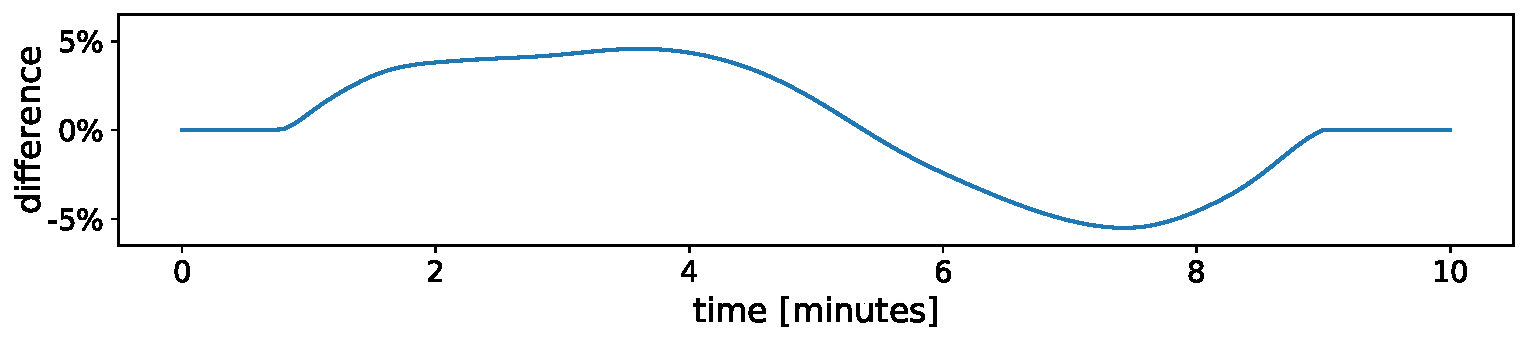
\includegraphics[width=\linewidth]{figures/earthsun_diff.pdf}
        \oscaption{earthsun}{%
            Mock secondary eclipse ingress light curves of the
            cloudless Earth expanded to spherical harmonic degree $l = 25$,
            viewed from an orientation where the Earth is occulted behind
            a solar latitude of $30^\circ$.
            Black curves show the analytic solution; orange dots correspond
            to brute force numerical integration on a grid of
            ${\sim}10^6$ points.
            The top panel shows the light curve in emitted light and is
            similar to Figure~13 in \citet{Luger2019}.
            The middle panel (this work) shows the same light curve in
            reflected light.
            The bottom panel shows the difference between the
            normalized reflected and emitted light curves.
            \label{fig:earthsun}
        }
    \end{centering}
\end{figure}

Our last sample light curve is Figure~\ref{fig:earthsun}, which shows
a secondary eclipse light curve of the Earth as it is occulted by the
Sun. The model for the Earth is the same as above, and the observer is
now close to the ecliptic, but slightly misaligned so that the
Earth is occulted behind a solar latitude of $30^\circ$ (i.e., at
a solar impact parameter of $0.5$). The observation takes place at the
June solstice, so the Earth is tilted by $23.5^\circ$ out of the page.
As before, the top panel shows the light curve in thermal light; this
is similar to the top panel of Figure~13 in \citet{Luger2019}. The orange
dots again correspond to the numerical solution.
%
The center panel shows the same light curve in reflected light.
Because the observation occurs very close to full phase, the normalized
light curves look very similar to each other.
The bottom panel shows the difference between the two
(reflected minus thermal), which is only on the order of a few percent.
%
In fact, because
the illumination profile is proportional to the cosine of the viewing
angle, $\mu$, and the reflection is assumed to be isotropic, the
(normalized) secondary eclipse light curve in reflected light is to
good approximation equal
to a limb-darkened thermal occultation light curve with
linear limb darkening coefficient $u_1 = 1$. As we will see later, for very
close-in planets this approximation breaks down, since the illumination
phases at secondary eclipse ingress and egress are sufficiently different
from full phase.

%

\subsection{Performance}
\label{sec:performance}

As we discuss in the Appendix, the model for phase curves and
occultation light curves in reflected light may be expressed
analytically in terms of purely algebraic and trigonometric functions
and in some cases incomplete elliptic integrals of the first, second,
and third kinds. We have derived efficient and numerically stable
recursion relations to compute the relevant expressions and their
derivatives. At times, these involve the evaluation of certain
expressions numerically, especially when doing so
leads to either a speed-up or a significant gain in numerical precision.
In particular, as we discuss in Appendix~\ref{sec:which-case}, the
integration boundaries during an occultation sometimes depend on the
solution to a quartic equation. While this can be solved in closed form,
the analytic solution can often be very unstable. We therefore solve
the quartic numerically, attaining a precision for the roots within a
few orders of magnitude of machine (double) precision.

Figures~\ref{fig:speed_no_occ} and \ref{fig:speed} summarize
the precision and computation time of the \starry algorithm for
two typical scenarios: a phase curve evaluation
(Figure~\ref{fig:speed_no_occ}) and an occultation evaluation
(Figure~\ref{fig:speed}).

\begin{figure}[p!]
    \begin{centering}
        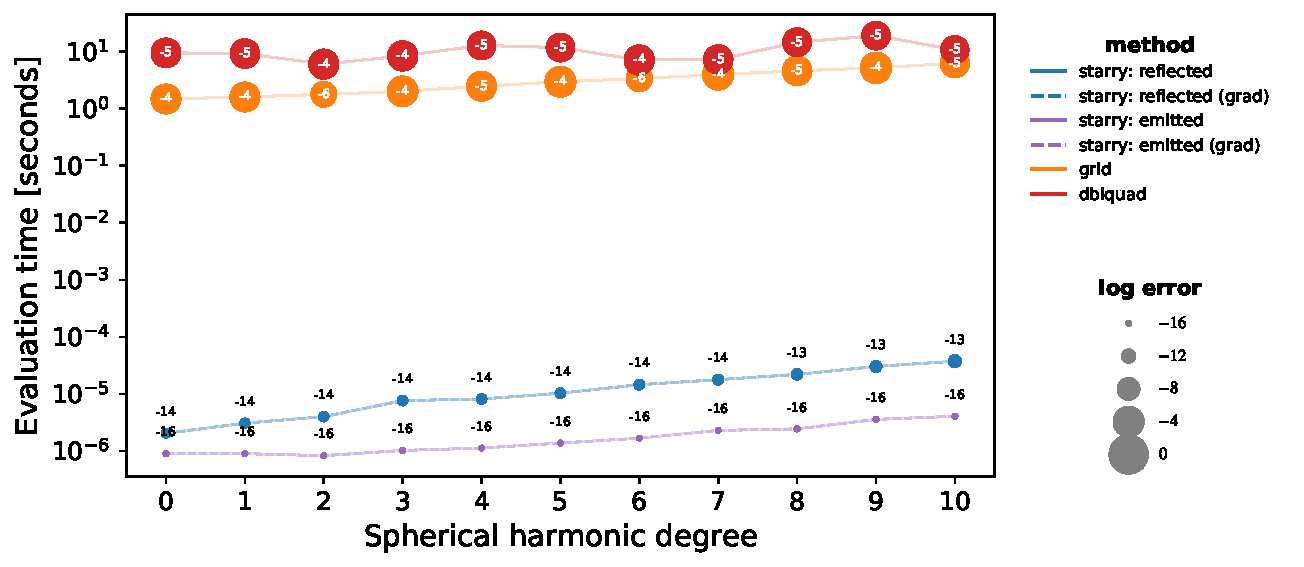
\includegraphics[width=\linewidth]{figures/speed_no_occ.pdf}
        \oscaption{speed}{%
            Evaluation time (vertical axis)
            and numerical precision (point size)
            for a single phase curve evaluation as a function of spherical
            harmonic degree for different methods.
            In purple we show results for the emitted light
            \starry algorithm from \citet{Luger2019} (solid: no gradient,
            dashed: with gradient), and in blue we show results for
            the reflected
            light algorithm from this paper (solid: no gradient,
            dashed: with gradient). For comparison, in orange we show
            results for discrete integration on a grid (solid) and
            numerical integration using two-dimensional Gaussian
            quadrature (dashed); neither of these include gradient
            evaluations. The reflected light algorithm is
            comparable in efficiency and precision to the emitted
            light algorithm. It is ${\sim}5$ orders of magnitude faster
            and ${\sim}10$ orders of magnitude more precise than numerical
            integration.
            \label{fig:speed_no_occ}
        }
    \end{centering}
\end{figure}

\begin{figure}[p!]
    \begin{centering}
        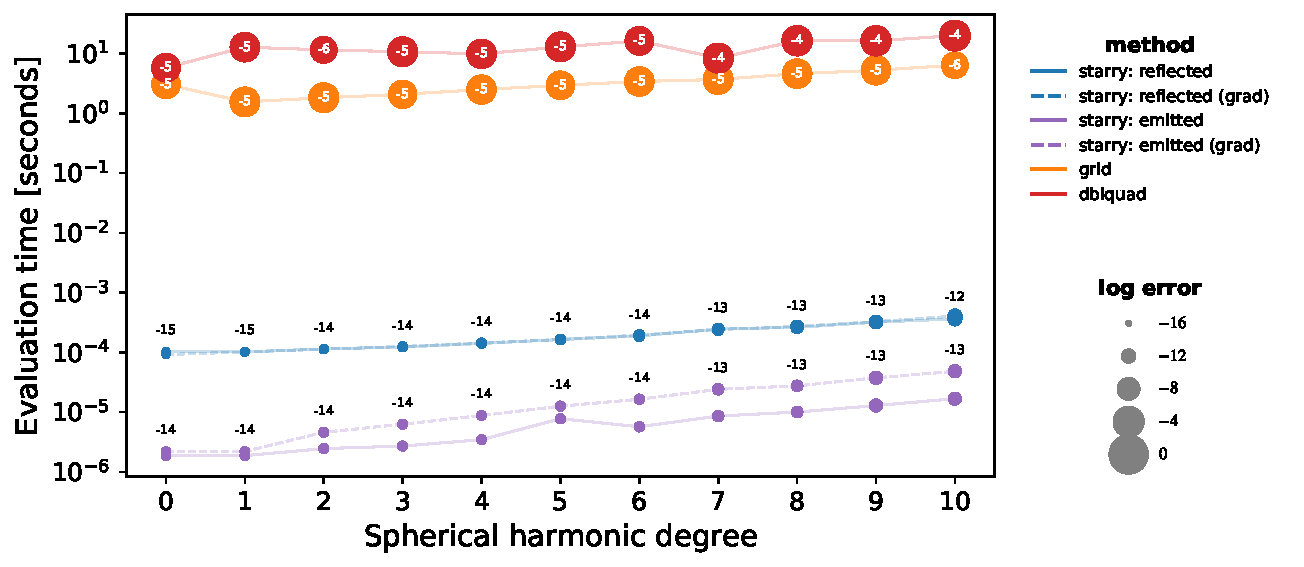
\includegraphics[width=\linewidth]{figures/speed.pdf}
        \oscaption{speed}{%
            Same as Figure~\ref{fig:speed_no_occ}, but for an occultation
            evaluation in which the occultor intersects the terminator
            (case 6 in Appendix~\ref{sec:solution-occ}).
            The reflected light algorithm is around one
            order of magnitude slower and comparably precise to the emitted
            light algorithm. It is ${\sim}4$ orders of magnitude faster
            and ${\sim}10$ orders of magnitude more precise than numerical
            integration.
            \label{fig:speed}
        }
    \end{centering}
\end{figure}

\subsection{Implementation and usage}
\label{sec:usage}

Hello.

% DEBUG
\clearpage

\section{Extensions}
\label{sec:extensions}

\subsection{Extended illumination source}
\label{sec:extended}
Planets to consider: 55 Cnc e, Kelt-9b.
Assuming $R_\star > R_p$, the angular extent of the terminator
past $\nicefrac{\pi}{2}$ is
%
\begin{proof}{}
    \label{eq:tau}
    \tau &= \arcsin\left( \frac{R_\star - R_p}{d} \right)
\end{proof}
%
where $R_\star$ is the radius of the star,
$R_p$ is the radius of the planet, and $d$ is the separation of their
centers.

For Kelt-9b, $\nicefrac{R_p}{R_\star} = 0.083$ and
$\nicefrac{a}{R_\star} = 3.16$, where $a$ is the semi-major axis of the
planet \citep{Wong2019}. Asssuming zero eccentricity and ignoring any
stellar oblateness
\citep[see][]{Ahlers2020}, we find that
the day/night terminator extends $\tau \approx 17^\circ$ past the limb
of the planet. Figure~\ref{fig:extended} shows...

\begin{figure}[ht!]
    \begin{centering}
        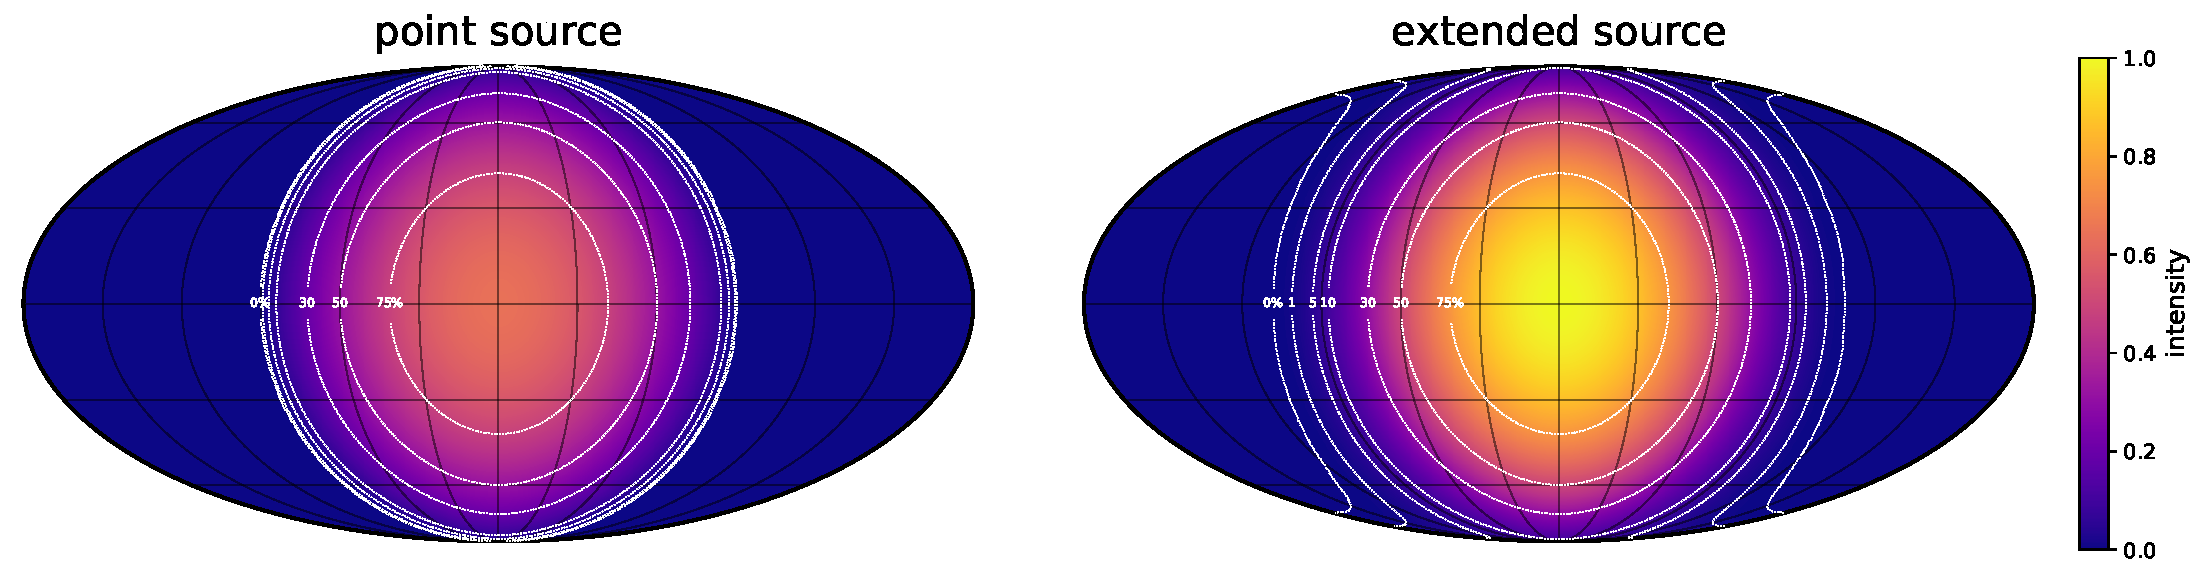
\includegraphics[width=\linewidth]{figures/extended.pdf}
        \oscaption{extended}{%
            Normalized surface intensity on Kelt-9b viewed in a
            Mollweide projection assuming a point illumination source
            (left) and accounting for the finite extent of the star
            (right). The day/night terminator extends about $17^\circ$
            past where it is in the point source case. The sub-stellar
            intensity is higher in the extended source case because the
            sub-planet point on the star is
            closer to the planet than in the case where the star is a point
            source located at the center of the star.
            \label{fig:extended}
        }
    \end{centering}
\end{figure}

Figure~\ref{fig:kelt9b} shows...

\begin{figure}[p!]
    \begin{centering}
        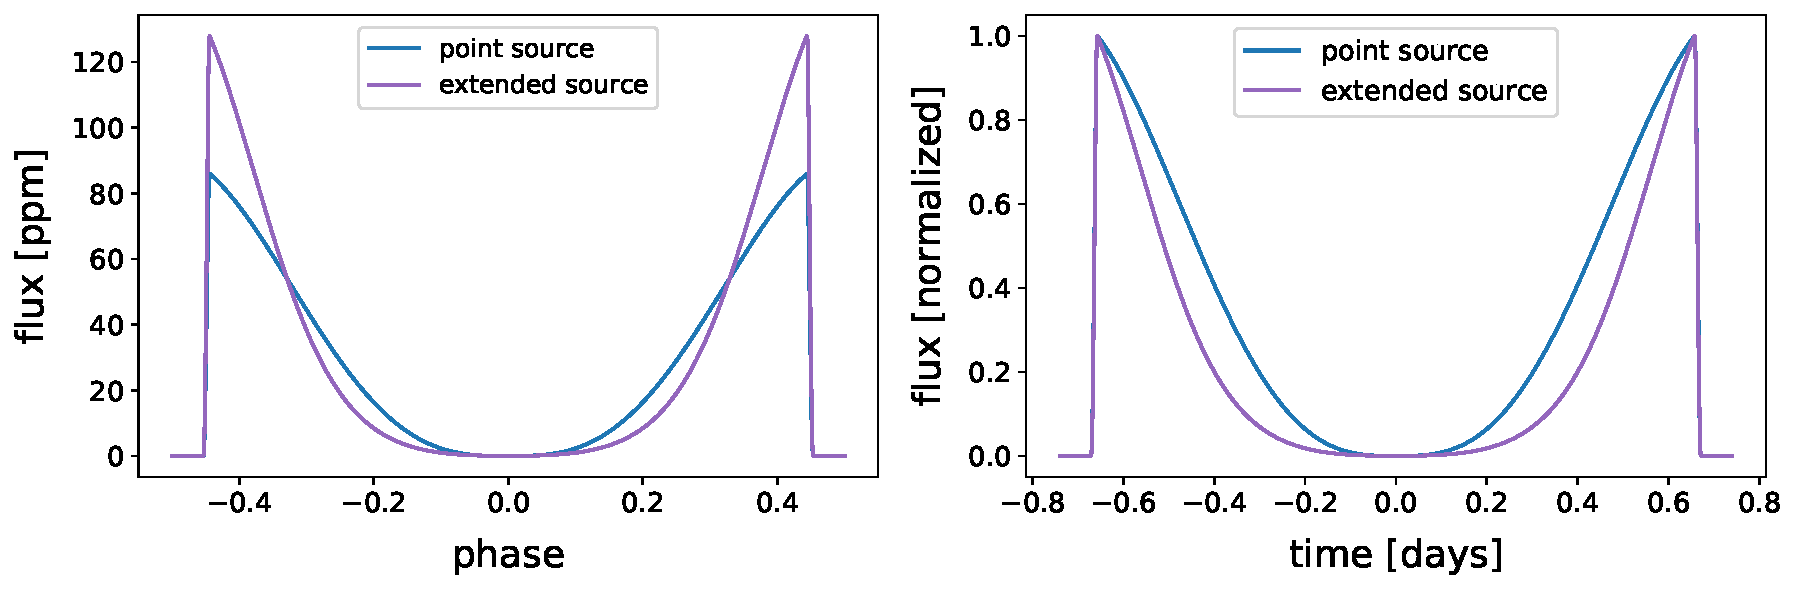
\includegraphics[width=\linewidth]{figures/kelt9b.pdf}
        \oscaption{kelt9b}{%
            Reflected light phase curve model for Kelt-9b, assuming
            a spherical albedo $A = 0.2$. The transit (phase zero)
            is not included. Blue is the \starry model
            assuming a point source illumination; purple accounts for
            the finite size of the star.
            The left panel shows the two models in parts per million
            of the stellar flux; the right panel shows the models
            normalized so their maximum value is unity.
            The primary effect of the extended source size is to
            increase the planet flux near full phase, since the stellar
            surface is on average slightly closer to the planet, and
            to change the overall curvature of the phase curve.
            The shape of secondary eclipse, however, is relatively
            insensitive to the point source approximation
            (see Figure~\ref{fig:kelt9b_eclipse}).
            \label{fig:kelt9b}
        }
    \end{centering}
\end{figure}

\begin{figure}[p!]
    \begin{centering}
        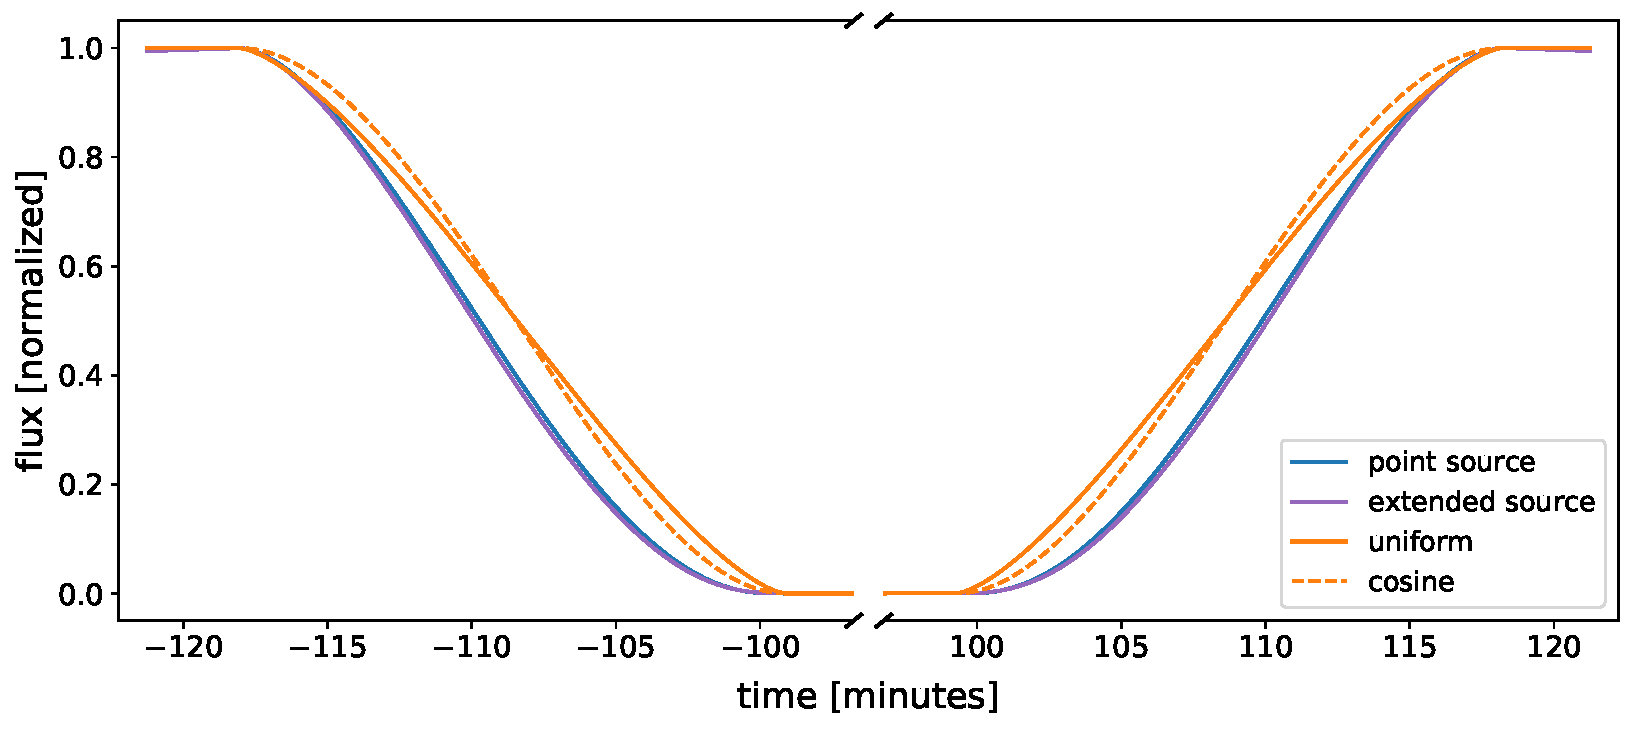
\includegraphics[width=\linewidth]{figures/kelt9b_eclipse.pdf}
        \oscaption{kelt9b}{%
            Normalized reflected light secondary eclipse model for Kelt-9b,
            assuming a spherical albedo $A = 0.2$. Blue is the \starry model
            assuming a point source illumination; purple accounts for
            the finite size of the star. The orange curves show
            approximate models computed using the \citet{MandelAgol2002}
            model: a sphere of uniform intensity (solid orange)
            and a sphere whose intensity falls as the cosine of the
            viewing angle from the center of the planet disk
            (dashed orange).
            Because Kelt-9b is so close to its host star, the illumination
            phase changes significantly from ingress to egress, and neither
            approximation accurately captures the behavior of the light curve.
            On the other hand, the point source approximation agrees well with
            the extended source solution, modulo an overall amplitude
            difference (see Figure~\ref{fig:kelt9b}).
            \label{fig:kelt9b_eclipse}
        }
    \end{centering}
\end{figure}

\subsection{Non-Lambertian scatterers}
\label{sec:nonlambertian}
Just change $\mathbf{I}$. \citep{OrenNayar1994}.

\begin{figure}[p!]
    \begin{centering}
        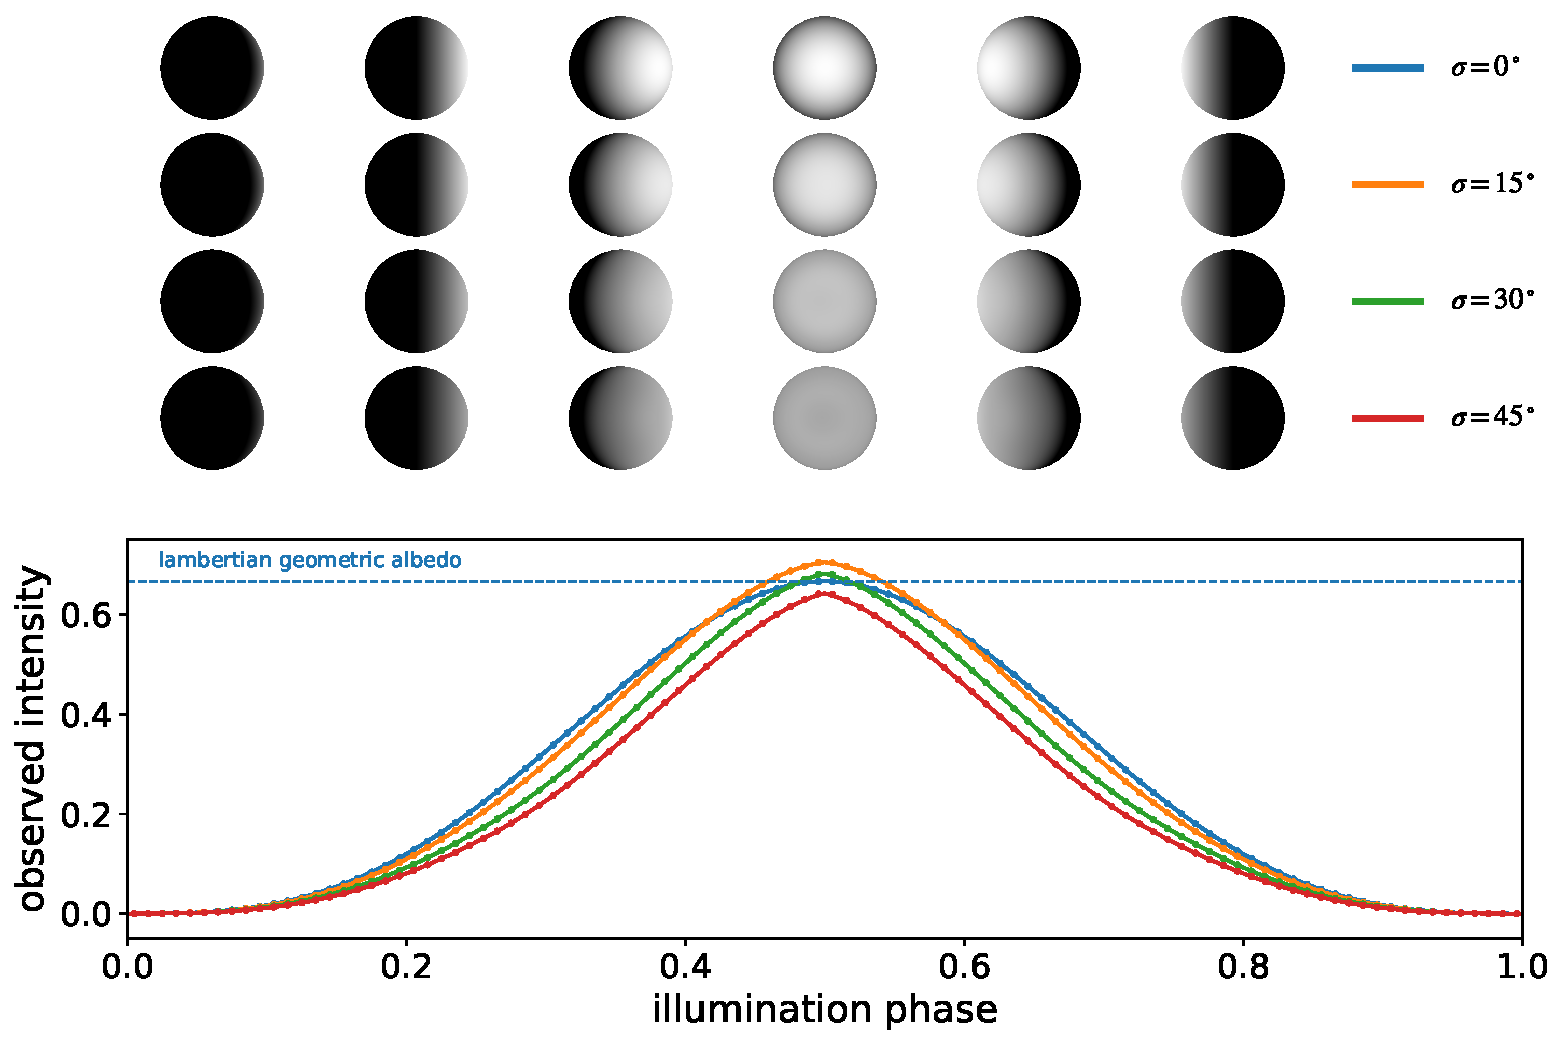
\includegraphics[width=\linewidth]{figures/oren_nayar.pdf}
        \oscaption{oren_nayar}{%
            Intensity measured from a sphere at varying illumination
            phase under the \citet{OrenNayar1994} scattering model.
            The top panel shows spheres rendered with different surface
            roughness coefficients ranging from $\sigma = 0^\circ$
            (the Lambertian case) to $\sigma = 45^\circ$. The bottom
            panel shows the corresponding phase curves for a sphere
            of unit spherical albedo illuminated by a point source
            at $r_s = 1$, computed
            analytically from a degree \STARRYQUADPOINTS expansion
            of the scattering law. Dots
            correspond to the intensity computed numerically directly
            from Equation~(30) in \citet{OrenNayar1994}.
            \label{fig:oren_nayar}
        }
    \end{centering}
\end{figure}
%

\section{Applications}
\label{sec:applications}

\begin{figure}[p!]
    \begin{centering}
        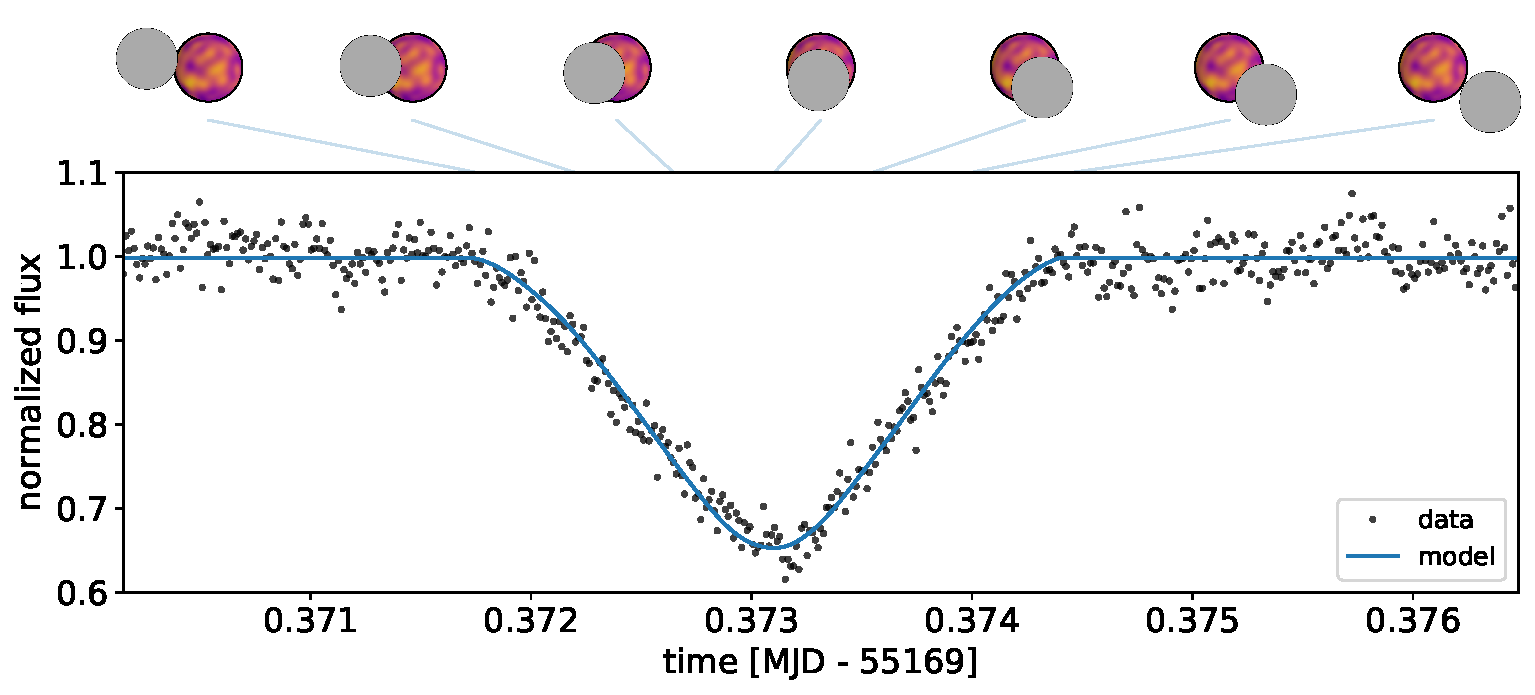
\includegraphics[width=\linewidth]{figures/io_europa.pdf}
        \oscaption{io_europa}{%
            Visible-light occultation of Io by Europa observed
            on 04 Dec 2009 by the PHEMU09 campaign \citep{Arlot2014}.
            The blue line is the \starry model, based of an
            $l=15$ spherical harmonic fit to the
            Galileio global color mosaic of Io \citep{Becker2005},
            an $l=\STARRYQUADPOINTS$ expansion of the
            \citet{OrenNayar1994} scattering law, and orbital
            information from the JPL Horizons \xxx{(cite)} database.
            See text for details.
            \label{fig:io_europa}
        }
    \end{centering}
\end{figure}
%

\subsection{Information}
\label{sec:information}

\pagebreak

% Bibliography
\bibliography{bib}


% APPENDIX
\appendix

%

\section{The Problem}
\label{sec:the-problem}
%
This paper closely follows the
notation and formalism introduced in \citet{Luger2019}. While we
include all of the relevant equations and definitions below,
the reader is encouraged to
review \citet{Luger2019} before proceeding.
To improve the readability of this paper,
Tables~\ref{tab:symbols}--\ref{tab:matrices} at the end list the principal
symbols and quantities used throughout the text, with links to the
sections and equations in which they are defined.

\subsection{Review of the \starry algorithm in emitted light}
\label{sec:starry-review}
%
Without loss of generality, assume the body whose flux we wish to compute
has radius unity and sits at the origin of a right-handed Cartesian coordinate
system in some frame $\mathcal{F}_0$. In this frame,
the surface (emitted) intensity field of the body is described by a
vector $\mathbf{y}$ of coefficients in the spherical harmonic
basis $\by$:
%
\begin{align}
    \label{eq:by}
    \by(x, y) & =
    \begin{pmatrix}
        Y_{0, 0}  &
        Y_{1, -1} & Y_{1, 0}  & Y_{1, 1} &
        Y_{2, -2} & Y_{2, -1} & Y_{2, 0} & Y_{2, 1} & Y_{2, 2} &
        \cdot\cdot\cdot
    \end{pmatrix}^\top
    \quad,
\end{align}
%
where the component at index $n$ is the spherical harmonic $Y_{l,m}(x, y)$ with
%
\begin{align}
    \label{eq:l-m}
    l & = \floor*{\sqrt{n}}
    \nonumber               \\
    m & = n - l^2 - l
    \quad.
\end{align}
%
The spherical harmonics are traditionally expressed in spherical coordinates,
but for our purposes
it is more conventient to express them in Cartesian coordinates on
the sky-projected disk, in which case they are simply polynomials in
$x$, $y$, and $z$ \citep[see Appendix~A in][]{Luger2019}.

An observer views the body from a large distance in the sky frame
$\mathcal{F}$, in which the $x$-axis points to the right,
the $y$-axis points up, and the $z$-axis points out of the sky
toward the observer. Following \citet{Luger2019}, if
an occultor of radius $r_o$ is located at sky position $(x_o, y_o)$,
we compute the visible flux $f$ from
%
\begin{align}
    \label{eq:sTARRy}
    f = \sTe \mathbf{A} \mathbf{R}' \mathbf{R} \mathbf{y}
    \quad,
\end{align}
%
where, from right to left, $\mathbf{R} = \mathbf{R}(\text{I}, \Lambda, \Theta)$
is a Wigner rotation matrix that rotates $\bvec{y}$ from $\mathcal{F}_0$
to the sky frame $\mathcal{F}$
given the body's inclination $\text{I}$, obliquity
$\Lambda$, and rotational phase $\Theta$
\citep[Appendix C in][]{Luger2019},
%
$\mathbf{R}' = \mathbf{R}'(x_o, y_o)$ rotates the body on the plane
of the sky into the integration frame $\mathcal{F}'$, in which the
occultor lies along the $+y'$-axis,
%
$\mathbf{A}$
\citep[Equation~B13 in][]{Luger2019}
is the change-of-basis matrix from $\by$
to the \emph{Green's basis} $\bg$ in which the integrals are computed,
whose component at index $n$ is
%
\begin{align}
    \label{eq:bg}
    \tilde{g}_{n}(x, y) & =
    \begin{dcases}
        %
        \frac{\mu+2}{2}x^\frac{\mu}{2} y^\frac{\nu}{2}
         & \qquad \mu, \nu \, \text{even}
        \\[1em]
        %
        z(x, y)
         & \qquad \mu = \nu = 1
        \\[1em]
        %
        3x^{l-2}yz(x, y)
         & \qquad \nu \, \text{odd}, \,
        \mu = 1, \,
        \frac{\mu + \nu}{2} \, \text{even}
        \\[1em]
        %
        z(x, y)
        \bigg(
        -x^{l-3} + x^{l-1} + 4x^{l-3}y^2
        \bigg)
         & \qquad \nu \, \text{odd}, \,
        \mu = 1, \,
        \, \text{odd}
        \\[1em]
        %
        z(x, y)
        \bigg(
        \frac{\mu-3}{2} x^\frac{\mu-5}{2} y^\frac{\nu-1}{2}
        \ - \
        \frac{\mu-3}{2} x^\frac{\mu-5}{2} y^\frac{\nu+3}{2}
        \\
        \qquad\qquad \ - \
        \frac{\mu+3}{2} x^\frac{\mu-1}{2} y^\frac{\nu-1}{2}
        \bigg)
         & \qquad \text{otherwise}
        \quad,
    \end{dcases}
\end{align}
%
with
%
\begin{align}
    \label{eq:mu-nu}
    \mu & \equiv l - m
    \nonumber          \\
    \nu & \equiv l + m
\end{align}
%
and
%
\begin{align}
    \label{eq:z}
    z(x, y) \equiv \sqrt{1 - x^2 - y^2}
    \quad,
\end{align}
%
and $\sTe = \sTe(b_o, r_o)$ is the vector of solutions to the integral over
the projected visible disk of the body for each term in $\bg$
\citep[Equation~26 in][]{Luger2019}, with $b_o = \sqrt{x_o^2 + y_o^2}$.

If instead no occultor is present, we compute the total
visible flux $f_0$ from this body as
%
\begin{align}
    \label{eq:rTA1Ry}
    f_0 = \rTe \mathbf{A_1} \mathbf{R}'' \mathbf{R} \mathbf{y}
    \quad,
\end{align}
%
where, as before, $\mathbf{R} = \mathbf{R}(\text{I}, \Lambda, \Theta)$
rotates the body from $\mathcal{F}_0$
to the sky frame $\mathcal{F}$,
%
$\mathbf{R}''$ rotates the body on the plane
of the sky into the integration frame
$\mathcal{F}''$%
\footnote{%
    In \citet{Luger2019}, $\mathcal{F}'' = \mathcal{F}'$, so
    this rotation is trivial: $\mathbf{R}''$ is just the identity matrix.
},
%
$\mathbf{A_1}$
\citep[Equation~B11 in][]{Luger2019}
is the change-of-basis matrix from the spherical harmonic
basis $\by$ to the \emph{polynomial basis} $\bp$ in which the integrals
are computed, whose component at index $n$ is
%
\begin{align}
    \label{eq:bp}
    \tilde{p}_n(x, y) & =
    \begin{dcases}
        x^\frac{\mu}{2} y^\frac{\nu}{2}
         & \qquad \mu, \nu \, \text{even}
        \\[1em]
        x^\frac{\mu-1}{2} y^\frac{\nu-1}{2} z(x, y)
         & \qquad \text{otherwise}
        \quad,
    \end{dcases}
\end{align}
%
and $\rTe$ is the vector of solutions to the integral over
the projected visible disk of the body for each term in $\bp$
\citep[Equation~19 in][]{Luger2019}.

\subsection{Adapting the algorithm to the reflected light case}
\label{sec:adapting-starry}
%
In order to compute light curves in reflected light, we must make two
modifications to the \starry algorithm. First,
the expressions above assume that the coefficient vector
$\mathbf{y}$ describes the \emph{emissivity} of the body, which (in the
absence of limb darkening) is assumed to be Lambertian, i.e., all points on the
surface emit equally in all directions.
Here, we wish to derive the solution for the flux in the case of Lambertian
reflectance, in which case the vector $\mathbf{y}$ is taken to describe the
spherical albedo of the surface, $A$.

Second, we must explicitly model the illumination of the body. We assume the
body is illuminated by a point-like source whose flux measured by the observer
is unity. In this case, the observed intensity at any
point on the surface is proportional to the cosine of the angle $\phi$ between
the incident light and the surface normal. Points for which
$\phi \ge \nicefrac{\pi}{2}$ are unilluminated and
therefore have an intensity of zero.
%
If the point-like illumination source is placed at sky coordinates
$(x_s, y_s, z_s)$ in units of the radius of the illuminated body,
the day/night terminator on the body is a half-ellipse
of semi-major axis unity that is fully described by its (signed) semi-minor
axis,
%
\begin{proof}{}
    \label{eq:b}
    b = -\frac{z_s}{r_s}
    \quad,
\end{proof}
%
where $r_s = \sqrt{x_s^2 + y_s^2 + z_s^2}$ is the distance to the source,
%
and the angle $\theta$ by which its semi-major axis is rotated away from the
$+x$-axis (a frame-dependent quantity, defined below).
Given this formulation, and assuming that
$r_s \gg 1$,
it is straightforward to show that the illumination
$\mathcal{I}$ at a point $(x, y)$ on the projected disk of the body is given
by the function
%
\begin{proof}{}
    \label{eq:illum}
    \mathcal{I}(b, \theta, r_s; x, y)&=
    \text{max}\bigg( 0, I(b, \theta, r_s; x, y) \bigg)
\end{proof}
%
where
%
\begin{proof}{}
    \label{eq:illum_poly}
    I(b, \theta, r_s; x, y) &= \frac{1}{\pi r_s^2}
    \bigg(
    -b_c\sin\theta x + b_c\cos\theta y - bz(x, y)
    \bigg)
\end{proof}
%
with $b_c \equiv \sqrt{1 - b^2}$ and $z(x, y) = \sqrt{1 - x^2 - y^2}$.
A quick note on the normalization of Equation~(\ref{eq:illum_poly}):
if we place the illumination source along the $+z$-axis at $(0, 0, 1)$,
the body is seen at full phase, so $b = -1$, $b_c = 0$, and
%
\begin{proof}{}
    \mathcal{I}_\text{full}(x, y) = \frac{\sqrt{1 - x^2 - y^2}}{\pi}
    \quad.
\end{proof}
%
Integrating this over the full disk, we obtain the reflected flux measured
by the observer if the body has unit spherical albedo,
%
\begin{proof}{}
    \mathcal{f}_\text{full} &=
    \int_{-1}^{1}
    \int_{-\sqrt{1 - x^2}}^{\sqrt{1 - x^2}}
    \frac{\sqrt{1 - x^2 - y^2}}{\pi}
    \,
    \dd y
    \,
    \dd x
    \nonumber \\[0.5em]
    &= \frac{2}{3}
    \quad,
\end{proof}
%
which is precisely the geometric albedo of a Lambert
sphere \citep[see, e.g.][]{Seager2010}.

In principle, our task is now straightforward: weight each of the
terms in the Green's basis (Equation~\ref{eq:bg}) and integrate them
over the visible portion of the body's disk to obtain the reflected
light solution vector, $\sT$. Unfortunately, the piecewise nature
of Equation~(\ref{eq:illum}) makes direct evaluation of these integrals
extremely difficult in practice.
%
We find that it is more tractable to weight our basis terms by
the function $I$ (Equation~\ref{eq:illum_poly}) and to modify the limits
of integration to exclude the nightside of the body, where $I$ is
(unphysically) negative.
%
In particular, since $I$ is just a polynomial in $x$, $y$, and $z(x, y)$, we
can express it as a vector $\mathbf{i}(b, \theta)$ in the polynomial basis $\bp$.
Recalling the structure of the basis (Equation~\ref{eq:bp}),
we may write
%
\begin{proof}{}
    \label{eq:ivec}
    \mathbf{i}(b, \theta, r_s) & =
    \frac{1}{\pi r_s^2}
    \begin{pmatrix}
        0              \\
        -b_c\sin\theta \\
        -b             \\
        b_c\cos\theta
    \end{pmatrix}
    \quad.
\end{proof}
%
This fact allows us to construct a linear operator $\mathbf{I}$ to weight a map
vector in the polynomial basis by the illumination profile.
If we think about how each of the terms in $\bp$ transforms under $\mathbf{I}$,
%
\\[1em]
%
\begin{minipage}{0.22\linewidth}
    \begin{align}
        \begin{pmatrix}
            1 \\
            0 \\
            0 \\
            0
        \end{pmatrix}
         & \pmb{\rightarrow}
        \begin{pmatrix}
            \bvec{i}_0 \\ %1
            \bvec{i}_1 \\ %x
            \bvec{i}_2 \\ %z
            \bvec{i}_3 \\ %y
            0          \\ %x^2
            0          \\ %xz
            0          \\ %xy
            0          \\ %yz
            0             %y^2
        \end{pmatrix}
        \nonumber
    \end{align}
\end{minipage}
%
\begin{minipage}{0.22\linewidth}
    \begin{align}
        \begin{pmatrix}
            0 \\
            1 \\
            0 \\
            0
        \end{pmatrix}
         & \pmb{\rightarrow}
        \begin{pmatrix}
            0          \\ %1
            \bvec{i}_0 \\ %x
            0          \\ %z
            0          \\ %y
            \bvec{i}_1 \\ %x^2
            \bvec{i}_2 \\ %xz
            \bvec{i}_3 \\ %xy
            0          \\ %yz
            0    %y^2
        \end{pmatrix}
        \nonumber
    \end{align}
\end{minipage}
%
\begin{minipage}{0.22\linewidth}
    \begin{align}
        \begin{pmatrix}
            0 \\
            0 \\
            1 \\
            0
        \end{pmatrix}
         & \pmb{\rightarrow}
        \begin{pmatrix}
            \bvec{i}_2  \\ %1
            0           \\ %x
            \bvec{i}_0  \\ %z
            0           \\ %y
            -\bvec{i}_2 \\ %x^2
            \bvec{i}_1  \\ %xz
            0           \\ %xy
            \bvec{i}_3  \\ %yz
            -\bvec{i}_2    %y^2
        \end{pmatrix}
        \nonumber
    \end{align}
\end{minipage}
%
\begin{minipage}{0.22\linewidth}
    \begin{align}
        \begin{pmatrix}
            0 \\
            0 \\
            0 \\
            1
        \end{pmatrix}
         & \pmb{\rightarrow}
        \begin{pmatrix}
            0          \\ %1
            0          \\ %x
            0          \\ %z
            \bvec{i}_0 \\ %y
            0          \\ %x^2
            0          \\ %xz
            \bvec{i}_1 \\ %xy
            \bvec{i}_2 \\ %yz
            \bvec{i}_3    %y^2
        \end{pmatrix}
        \nonumber
    \end{align}
\end{minipage}
\begin{minipage}{0.05\linewidth}
    \begin{align}
    \end{align}
\end{minipage}
%
\\[1em]
%
we can compose $\mathbf{I}$ out of these column vectors:
%
\begin{proof}{}
    \label{eq:Imat}
    \mathbf{I}(b, \theta, r_s) & =
    \frac{1}{\pi r_s^2}
    \begin{pmatrix}
        0              & 0              & -b             & 0              & \cdots \\
        -b_c\sin\theta & 0              & 0              & 0              & \cdots \\
        -b             & 0              & 0              & 0              & \cdots \\
        b_c\cos\theta  & 0              & 0              & 0              & \cdots \\
        0              & -b_c\sin\theta & b              & 0              & \cdots \\
        0              & -b             & -b_c\sin\theta & 0              & \cdots \\
        0              & b_c\cos\theta  & 0              & -b_c\sin\theta & \cdots \\
        0              & 0              & b_c\cos\theta  & -b             & \cdots \\
        0              & 0              & b              & b_c\cos\theta  & \cdots \\
        \vdots         & \vdots         & \vdots         & \vdots         & \ddots
    \end{pmatrix}
\end{proof}
%
where the dimensions of the matrix are $\big((l + 2)^2, (l + 1)^2\big)$, where
$l$ is the spherical harmonic degree of the map (this operator raises the
degree of the map by one).
%
Note, again, that this weighting is valid only on the dayside
hemisphere (see Equation~\ref{eq:illum}), as the operator $\mathbf{I}$ weights
points on the nightside by a \emph{negative} amount, which is clearly
unphysical. As we will see momentarily, we account for this by excluding the
nightside from the integration region in our flux integrals.

\begin{figure}[t!]
    \begin{centering}
        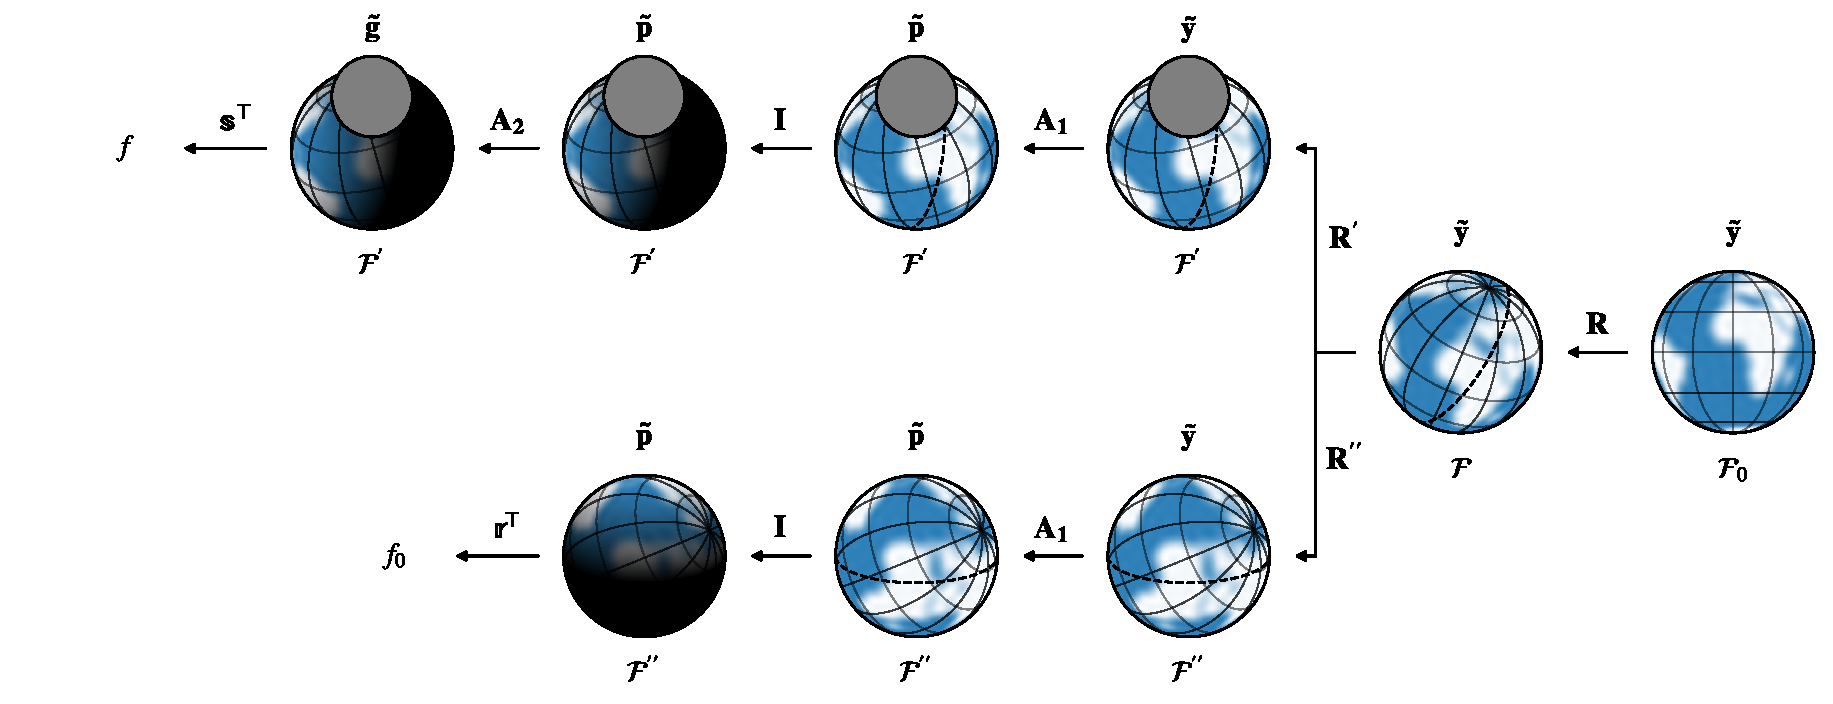
\includegraphics[width=\linewidth]{figures/frames.pdf}
        \oscaption{frames}{%
            How \starry computes the flux from a body in reflected light,
            tracking each of the linear transformations from the input map
            (far right) to the output (far left). The label below each map
            denotes the reference frame, while the label above
            each map denotes the basis in which the map is represented.
            Arrows indicate linear operations and are labeled accordingly.
            The upper branch corresponds to the occulted case
            (Equation~\ref{eq:sTA2IA1RRy}), while the
            lower branch corresponds to the case where the body
            is unocculted (Equation~\ref{eq:rTIA1RRy}).
            See text for details.
            \label{fig:frames}
        }
    \end{centering}
\end{figure}

We may now re-write Equations~(\ref{eq:sTARRy}) and (\ref{eq:rTA1Ry}) to
account for this illumination transformation. The flux during an occultation
is now given by
%
\begin{align}
    \label{eq:sTA2IA1RRy}
    f & =
    \sT(b, \theta', b_o, r_o)
    \mathbf{A_2}
    \mathbf{I}(b, \theta', r_s)
    \mathbf{A_1}
    \mathbf{R}'(x_o, y_o)
    \mathbf{R}(\text{I}, \Lambda, \Theta)
    \mathbf{y}
    \quad,
\end{align}
%
where
%
\begin{align}
    \label{eq:theta'}
    \theta' = \atantwo(x_o, y_o) - \atantwo(x_s, y_s)
\end{align}
%
is the angle of the terminator in the frame $\mathcal{F}'$.
Note that we made use of the fact that
$\mathbf{A} = \mathbf{A_2} \mathbf{A_1}$
\citep[Equation~14 in][]{Luger2019}, where $\mathbf{A_1}$ transforms from
the spherical harmonic basis $\by$ to the polynomial basis $\bp$, and
$\mathbf{A_2}$ transforms from $\bp$ to the Green's basis $\bg$.

Similarly, the flux when there is no occultation is now given by
%
\begin{align}
    \label{eq:rTIA1RRy}
    f_0 & =
    \rT(b)
    \mathbf{I}(b, \theta'', r_s)
    \mathbf{A_1}
    \mathbf{R}''(x_s, y_s)
    \mathbf{R}(\text{I}, \Lambda, \Theta)
    \mathbf{y}
    \quad,
\end{align}
%
where
%
\begin{align}
    \label{eq:theta''}
    \theta'' = 0
\end{align}
%
is the angle of the terminator in the frame $\mathcal{F}''$, by
construction. The transformation
$\mathbf{R}'' = \mathbf{R}''(x_s, y_s)$ rotates
the body
through an angle $\atantwo(x_s, y_s)$
so the semi-major axis of the terminator is aligned
with the $x''$-axis; as will become clear in \S\ref{sec:solution-no-occ} below,
this greatly simplifies the integration step.

Note that in both equations we replaced the integral vectors
$\rTe$ and $\sTe(b_o, r_o)$
with the vectors
$\rT(b)$ and $\sT(b, \theta', b_o, r_o)$,
respectively.
As we mentioned above, we must modify the integration limits to exclude the
nightside, where the weighting by $\mathbf{I}$ is unphysical.
The vectors $\rT$ and $\sT$ correspond to these
modified integrals, which we devote the rest of this paper to
computing.

Figure~\ref{fig:frames} summarizes the transformations involved in the two
equations above. Starting on the right with a map vector $\mathbf{y}$ in
the spherical harmonic basis $\by$, defined in some observer-independent frame
$\mathcal{F}_0$, we first rotate it via $\mathbf{R}$ to the sky frame
$\mathcal{F}$, in which the body is viewed by the
observer. If an occultor is present (upper branch of the figure),
we rotate the map from $\mathcal{F}$ via $\mathbf{R}'$ to the frame
$\mathcal{F}'$, in which the occultor lies along the
$+y'$-axis. We then apply $\mathbf{A_1}$ to change basis to $\bp$ and $\mathbf{I}$
to weight the map by the illumination. Finally, we change basis
via $\mathbf{A_2}$ to the Green's basis, in which we compute and dot the
integrals $\sT$.
If, on the other hand, there is no occultation (lower branch of the figure),
we instead rotate the map via $\mathbf{R}''$ to the integration frame
$\mathcal{F}''$, in which the terminator is parallel to the
$x''$-axis. We then apply $\mathbf{A_1}$ to change basis to $\bp$, apply the
illumination transform $\mathbf{I}$, and finally dot in the solutions to the
surface integrals $\rT$.

%

\section{The Solution: No Occultation}
\label{sec:solution-no-occ}
%
Before we tackle configurations involving occultations, we must address the
simpler problem of computing the total visible flux from an unocculted
body in reflected light (Equation~\ref{eq:rTIA1RRy}). This problem was
originally solved by \citet{Haggard2018} and subsequently by
\citet{Luger2019b}, but for completeness we present the detailed
derivation in the \starry formalism here.

As we discussed above, we perform the integration in a frame
$\mathcal{F}''$
in which the semi-major axis of the terminator is aligned with the
$x''$-axis, with the illumination source at $y'' \ge 0$.
The solution vector may then be computed from
%
\begin{align}
    \label{eq:rT}
    \rT(b) & =
    \int_{-1}^{1}
    \int_{b\sqrt{1 - x''^2}}^{\sqrt{1 - x''^2}}
    \bp(x'', y'')
    \ \dd y'' \ \dd x''
    \quad,
\end{align}
%
which is identical to Equation~(20) in \citet{Luger2019} except for the
lower integration limit of the inner integral. The lower limit is now
the equation describing the terminator, which ensures we always exclude the
nightside from the integration region.
%
For computational efficiency, in practice we compute the integral of the
intensity-weighted basis directly,
%
\xxx{NO LONGER TRUE. FIX THIS DEFINITION.}
%
\begin{align}
    \label{eq:rTI}
    \overset{\quad\pmb{\wedge}}{\mathbbb{r}}{^\top}(b, r_s) & \equiv
    \rT(b) \mathbf{I}(b, \theta'', r_s)
    \nonumber                                                        \\
                                                            & =
    \int_{-1}^{1}
    \int_{b\sqrt{1 - x''^2}}^{\sqrt{1 - x''^2}}
    \bp(x'', y'')
    \mathbf{I}(b, 0, r_s)
    \ \dd y'' \ \dd x''
    \quad,
\end{align}
%
recalling that in frame $\mathcal{F}''$, $\theta'' = 0$ by
definition.
%
Equation~(\ref{eq:rTI}) may be solved analytically in terms of purely
trigonometric and algebraic functions of $b$.
The component of $\overset{\quad\pmb{\wedge}}{\mathbbb{r}}{^\top}$
at index $n$ is given by
%
\begin{proof}{}
    \label{eq:rTsoln}
    \overset{\quad\wedge}{\mathbb{r}}_n(b, r_s) & =
    \frac{1}{\pi r_s^2}
    \begin{cases}
        \frac{b_c\left(1 - b^{\frac{\nu + 4}{2}}\right)}{2}
        \mathbb{L}_{\frac{\mu}{2}, \frac{\nu + 2}{2}} -
        b \mathbb{k}_\frac{\nu}{2}(b) \mathbb{M}_{\frac{\mu}{2}, \frac{\nu}{2}}
        %
         &
        %
        \qquad
        \mu, \nu \ \text{even}
        %
        \\[1em]
        %
        b_c
        \mathbb{k}_{\frac{\nu + 1}{2}}(b) \mathbb{M}_{\frac{\mu - 1}{2}, \frac{\nu + 1}{2}}
        %
        \\[0.5em]
        \qquad
        %
        - \frac{b}{2} \bigg\{
        \left(1 - b^{\frac{\nu + 1}{2}}\right)
        \left(
        \mathbb{L}_{\frac{\mu - 1}{2}, \frac{\nu - 1}{2}} -
        \mathbb{L}_{\frac{\mu + 3}{2}, \frac{\nu - 1}{2}}
        \right)
        \\[0.5em]
        \qquad\qquad
        -
        \left(1 - b^{\frac{\nu + 5}{2}}\right)
        \mathbb{L}_{\frac{\mu - 1}{2}, \frac{\nu + 3}{2}}
        \bigg\}
        %
         &
        %
        \qquad
        \text{otherwise}
        %
    \end{cases}
\end{proof}
%
where the components of $\mathbbb{k}$, $\mathbbb{L}$, and $\mathbbb{M}$
are given by
%
\begin{proof}{}
    \label{eq:HJK}
    \mathbb{k}_{j}(b) &= \int_b^1 a^j \sqrt{1 - a^2} \dd a
    \nonumber \\
    %
    \mathbb{L}_{i,j} &=
    \frac{
        \Gamma\left(\frac{i + 1}{2}\right)
        \Gamma\left(\frac{j + 1}{2}\right)
    }
    {
        \Gamma\left(\frac{i + j + 4}{2}\right)
    }
    %
    \nonumber \\
    %
    \mathbb{M}_{i,j} &=
    \frac{
        \Gamma\left(\frac{i + 1}{2}\right)
        \Gamma\left(\frac{j + 4}{2}\right)
    }
    {
        \Gamma\left(\frac{i + j + 5}{2}\right)
    }
    \quad,
\end{proof}
%
where $\Gamma$ is the gamma function.
%
Given initial conditions
%
\\[1em]
\begin{minipage}{.33\linewidth}
    \begin{align}
        \mathbb{k}_{0}(b) & = \frac{\arccos(b) - bb_c}{2}
        %
        \nonumber                                         \\
        %
        \mathbb{k}_{1}(b) & = \frac{b_c^3}{3}
        %
        \nonumber
    \end{align}
\end{minipage}%
\begin{minipage}{.32\linewidth}
    \begin{align}
        \mathbb{L}_{0,0} & = \pi
        %
        \nonumber                        \\
        %
        \mathbb{L}_{0,1} & = \frac{4}{3}
        %
        \nonumber
    \end{align}
\end{minipage}%
\begin{minipage}{.33\linewidth}
    \begin{proof}{}
        \label{eq:IJK0}
        \mathbb{M}_{0,0} &= \frac{4}{3}
        %
        \nonumber \\
        \mathbb{M}_{0,1} &= \frac{3\pi}{8}
    \end{proof}
\end{minipage}
\\[1em]
%
we may compute all higher order terms from the recurrence relations
%
\begin{proof}{}
    \label{eq:IJKrec}
    \mathbb{k}_{j}(b) &= \frac{b^n b_c^3 + (j - 1) \mathbb{k}_{j - 2}(b)}{j + 2}
    %
    \nonumber \\
    %
    \mathbb{L}_{0,j} &= \left(\frac{j - 1}{j + 2}\right) \mathbb{L}_{0,j-2}
    %
    \nonumber \\
    %
    \mathbb{M}_{0,j} &= \left(\frac{j + 2}{j + 3}\right) \mathbb{M}_{0,j-2}
    %
    \nonumber \\
    %
    \mathbb{L}_{i,j} &= \left(\frac{i - 1}{i + j + 2}\right) \mathbb{L}_{i-2,j}
    %
    \nonumber \\
    %
    \mathbb{M}_{i,j} &= \left(\frac{i - 1}{i + j + 3}\right) \mathbb{M}_{i-2,j}
    \quad.
\end{proof}
%
Once $\overset{\quad\pmb{\wedge}}{\mathbbb{r}}{^\top}$ is known,
the observed flux is computed from
(c.f. Equation~\ref{eq:rTIA1RRy})
%
\begin{proof}{}
    \label{eq:f0}
    f_0 & =
    \overset{\quad\pmb{\wedge}}{\mathbbb{r}}{^\top}(b, r_s)
    \mathbf{A_1}
    \mathbf{R}''(x_s, y_s)
    \mathbf{R}(\text{I}, \Lambda, \Theta)
    \mathbf{y}
    \quad.
\end{proof}
%
Finally, for future reference, we can also compute what we will call the
\emph{complement} of case 0:
%
\begin{proof}{}
    \label{eq:f0hat}
    \hat{f}_0 & =
    -\overset{\quad\pmb{\wedge}}{\mathbbb{r}}{^\top}(-b, r_s)
    \mathbf{A_1}
    \mathbf{R}''(-x_s, -y_s)
    \mathbf{R}(\text{I}, \Lambda, \Theta)
    \mathbf{y}
    \quad,
\end{proof}
%
\xxx{FIX THIS DEFINITION. NO LONGER HOW WE COMPUTE IT.}
%
This is the flux we would get if we placed a \emph{negative} illumination
source at the antipode $(-x_s, -y_s, -z_s)$ of the true source, and
will be useful in negating the unphysical negative contribution from our
polynomial illumination function (Equation~\ref{eq:illum_poly}) in
the following section.

\section{The Solution: Occultation}
\label{sec:solution-occ}
%
The integration in the unocculted case presented above is relatively
straightforward, since
the boundaries of integration are always the half-ellipse defining the
terminator and the half-circle defining the upper limb of the body
(Equation~\ref{eq:rT}). When an occultor is present, however, the
integration boundaries are far less trivial, since they may or may not
include sections of the terminator, sections of the limb of the body,
and sections of the limb of the occultor. The integration regions may also
be disjoint; for instance, in case 7 of Figure~\ref{fig:cases}, the
portion of the dayside that is unocculted consists of two separate
regions.

Whereas in \citet{Luger2019} we compute the observed flux by always
integrating over the unocculted portion of the disk, here we find that
it is often easier and more computationally efficient to compute the
integral of the intensity over the
\emph{simplest} region -- meaning the one with the fewest boundaries --
and combine it with the formalism from \S\ref{sec:solution-no-occ} to
compute the visible flux. These integrals may be over the unocculted dayside,
the occulted dayside, the unocculted nightside, or the occulted nightside;
in the case of the latter three, a bit of algebra
(\S\ref{sec:cases-pathological}--\S\ref{sec:cases-pathological}) is needed
to relate these to the observed flux. Additionally, in some cases we can
avoid computing new integrals entirely, as the solution can be obtained from
a combination of the classical \starry solution vector $\sT$ and the
formalism from the unocculted case (\S\ref{sec:solution-no-occ}).

After exhaustive experimentation, we identified in total 14 families of
geometrical configurations for the occultation problem,
each defined by a distinct combination of integration
boundaries; these are shown in Figures~\ref{fig:cases} and
\ref{fig:pathological}.
Together, these cases encompass all possible
occultation configurations, for any illumination angle, occultor size, and
occultor position.

Before we discuss how to compute the occultation integrals, we must first
develop a procedure to identify the relevant case given the occultor
impact parameter $b_o = \sqrt{x_o^2 + y_o^2}$ and radius $r_o$ and
the terminator semi-minor
axis $b$ and angle $\theta'$ in the frame $\mathcal{F}'$.
Then, once the case is determined, we must
identify the relevant integration boundaries, which depend on the points
of intesection between the limb of the body, the limb of the occultor, and
the terminator. We do so in the following sections.

%

\subsection{Case determination}
\label{sec:which-case}

\begin{figure}[t!]
    \begin{centering}
        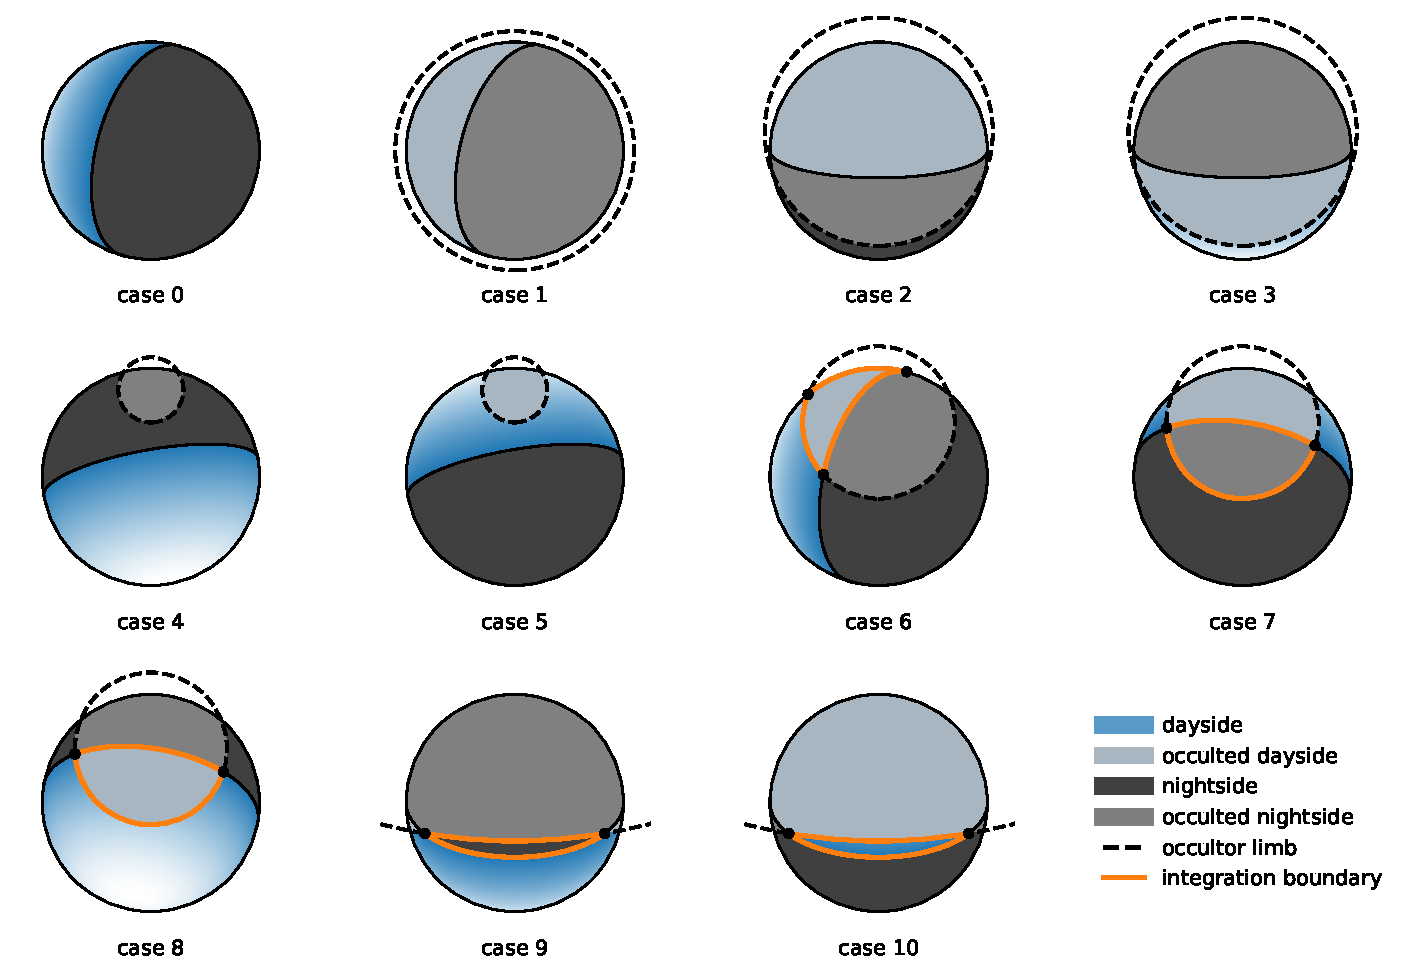
\includegraphics[width=\linewidth]{figures/cases.pdf}
        \oscaption{cases}{%
            The 10 principal families of cases of occultations in
            reflected light.
            In these figures, the body with the solid outline
            is the one whose flux we are interested in, and the body with the
            dashed outline is the occultor.
            The nightside of the occulted body is colored
            black (dark grey if occulted), and the dayside is colored blue
            (bluish-grey if occulted).
            Case 0 is the unocculted case (\S\ref{sec:solution-no-occ}),
            while cases 1--5 involve
            configurations in which the limb of the occultor does not intersect
            with the terminator at any point, so the visible flux may be
            computed in terms of classical \starry integrals. The remaining
            cases require integration along the orange boundary (the curves
            $\mathcal{P}$, $\mathcal{T}$, and $\mathcal{Q}$ of
            \S\ref{sec:cases-hard}), which
            include the terminator. These involve the evaluation of incomplete
            elliptic integrals and are derived below.
            \label{fig:cases}
        }
    \end{centering}
\end{figure}

The key to identifying the case corresponding to a given configuration is
to determine whether or not the limb of the occultor intersects the terminator
of the body, and if so, the points of intersection.
While we perform the integration in frame $\mathcal{F}'$, finding the points
of intersection with the terminator is easier if we temporarily switch to
the frame $\mathcal{F}''$, in which the terminator
is parallel to the $x''$-axis.
In this frame, the equations defining the terminator and the limb of the
occultor are, respectively,
%
\begin{proof}{}
    y''_1(x'') & = b \sqrt{1 - x''^2}
    \nonumber                                               \\
    y''_2(x'') & = y''_o \pm \sqrt{r_o^2 - (x'' - x''_o)^2}
\end{proof}
%
where
%
\begin{proof}{}
    x''_o = b_o\sin\theta'
    \nonumber \\
    y''_o = b_o\cos\theta'
\end{proof}
%
are the coordinates of the occultor in $\mathcal{F}''$.
%
We wish to find the vector of $N$ points
$\mathbf{x''} = \left(x_0, x_1, {\cdot\cdot\cdot}, x_{N-1}\right)^\top$
for which
$y''_1(x_n'') - y''_2(x_n'') = 0$. Following \citet{Luger2017}, we may
express this condition as the quartic equation
%
\begin{proof}{}
    \label{eq:quartic}
    A {x''}^4 + B {x''}^3 + C {x''}^2 + D {x''} + E = 0
\end{proof}
%
with coefficients
%
\begin{proof}{}
    \label{eq:quartic-coeffs}
    A &= (1 - b^2)^2
    \nonumber \\
    B &= -4 x''_o (1 - b^2)
    \nonumber \\
    C &= -2 \bigg(
    b^4
    + r_o^2
    - 3 {x''_o}^2
    - {y''_o}^2
    - b^2 \big(1 + r_o^2 - {x''_o}^2 + {y''_o}^2\big)
    \bigg)
    \nonumber \\
    D &= -4 x''_o (b^2 - r_o^2 + {x''_o}^2 + {y''_o}^2)
    \nonumber \\
    E &=
    b^4
    - 2 b^2 \big(r_o^2 - {x''_o}^2 + {y''_o}^2\big)
    + \big(r_o^2 - {x''_o}^2 - {y''_o}^2\big)^2
    \quad.
\end{proof}
%
Although closed-form solutions to quartic equations exist
\citep[see, e.g.,][who solve for the area of overlap between two ellipses
    analytically]{Hughes2011}, they are prone to significant numerical
instabilities. Instead, we solve for the roots of the quartic
numerically by casting it
as an eigenvalue problem \citep[e.g.,][]{Edelman1995} and polish the
results with a few iterations of Newton's method. We find that this is
reasonably computationally efficient and
yields roots with precision within a couple orders of magnitude of machine
epsilon (see \S\ref{sec:performance}).

In general, the quartic defined by Equation~(\ref{eq:quartic}) has
$N=4$ (potentially degenerate) roots, some of which may be complex, and some
of which correspond to intersections with the wrong half of the
terminator ellipse (i.e., the section of the terminator on the far side
of the body). After excluding the unphysical solutions, we are still left with
anywhere between zero and four roots.

Cases with zero roots (case 1 -- case 4) are treated in \S\ref{sec:cases-easy},
while cases with one or two roots (case 5 -- case 8) are treated in
\S\ref{sec:cases-hard}. Cases with three or four roots
(case 9 -- case 10) are rarely encountered
in practice, but are possible for some pathological configurations; these are
treated in \S\ref{sec:cases-pathological}.

%

\subsection{Cases 1--5}
\label{sec:cases-easy}
%
Cases 1--5 (see Figure~\ref{fig:cases}) involve configurations in which the
occultor does not intersect with
the terminator of the occulted body, and are therefore fairly
straightforward to solve. In particular, we can use the original emitted
light solution from \citet{Luger2019}, provided we weight the map by our
polynomial illumination function:
%
\begin{proof}{}
    \label{eq:fI}
    f_I &=
    \sTe(b_o, r_o)
    \mathbf{A_2}
    \mathbf{I}(b, \theta', r_s)
    \mathbf{A_1}
    \mathbf{R}'(x_o, y_o)
    \mathbf{R}(\text{I}, \Lambda, \Theta)
    \mathbf{y}
    \quad,
\end{proof}
%
where $\sTe(b_o, r_o)$ is the emitted light solution vector
\citep[Equation~26 in][]{Luger2019}. The flux $f_I$ is the flux one would
measure from a body whose surface map is weighted by the illumination function
$\mathbf{I}(b, \theta', r_s)$ during an occultation. Note that this is not
necessarily the \emph{observed} flux, since this may include the unphysical
negative contribution from the nightside. We must compute the actual
observed flux on a case-by-case basis.

Case 1 corresponds to any complete occultation of the body
($b_o \le r_o - 1$), so the solution for the flux is trivial:
%
\begin{align}
    \label{eq:f1}
    f_1 = 0
    \quad.
\end{align}
%
Case 2 corresponds to occultations in which the occultor blocks \emph{all} of
the dayside of the body and \emph{some} of the nightside. In this
configuration, the unocculted part of the disk consists only of nightside, so
the solution is again trivial:
%
\begin{align}{}
    \label{eq:f2}
    f_2 = 0
    \quad.
\end{align}
%
Conversely, case 3 corresponds to occultations in which the occultor blocks
\emph{all} of the nightside of the body and \emph{some} of the dayside.
Since the visible portion of the disk consistss only of dayside, we can
simply use the weighted solution in emitted light
(Equation~\ref{eq:fI}):
%
\begin{proof}{}
    \label{eq:f3}
    f_3 = f_I
\end{proof}
%
Case 4 involves any occultation in which the occultor blocks \emph{only} the
nightside of the body (regardless of whether or not it intersects with the
limb of the body). Since the nightside intensity is zero everywhere, this case
is also trivial, as the flux is equal to the flux in the no occultation case
(Equation~\ref{eq:f0}):
%
\begin{align}
    \label{eq:f4}
    f_2 = f_0
    \quad.
\end{align}
%
Finally, case 5 involves any occultation in which the occultor blocks
\emph{only} the dayside of the body (regardless of whether or not it
intersects with the limb). We first compute the illumination-weighted flux
$f_I$ as above, then negate the unphysical nightside contribution
using Equation~(\ref{eq:f0hat}):
%
\begin{proof}{}
    \label{eq:f5}
    f_5 = f_I - \hat{f}_0
    \quad.
\end{proof}

%

\subsection{Cases 6--10}
\label{sec:cases-hard}
%

\begin{figure}[t!]
    \begin{centering}
        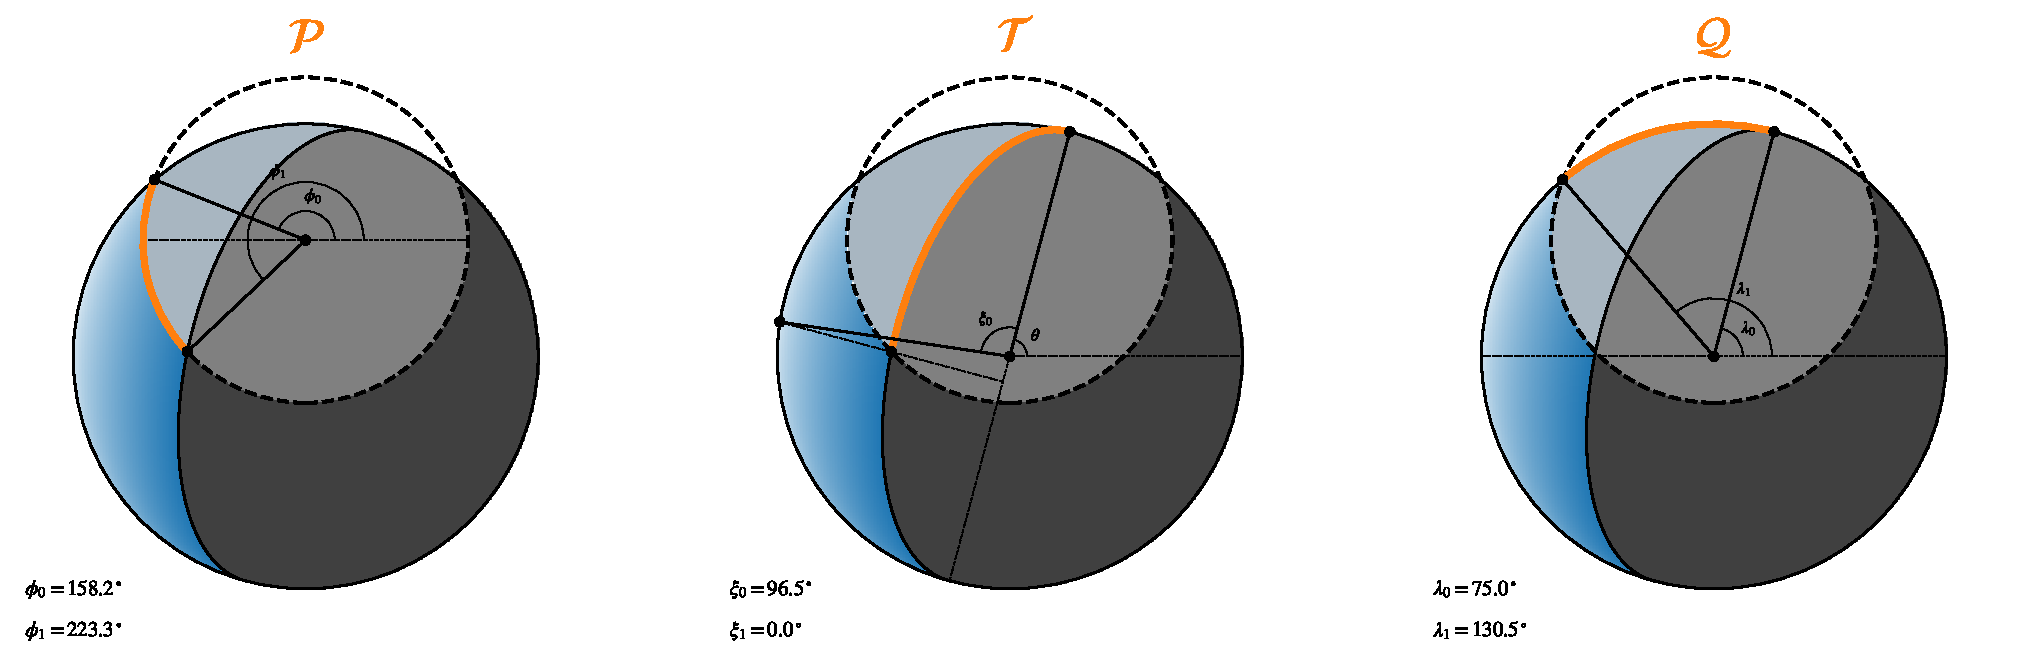
\includegraphics[width=\linewidth]{figures/geometry.pdf}
        \oscaption{geometry}{%
            Geometry of an occultation in reflected light, corresponding
            to case 6 in Figure~\ref{fig:cases}. The surface integral over
            the occulted portion of the dayside (bluish-grey region)
            is computed from the line integrals of the antiderivatives of the
            surface intensity map along the boundary curves
            $\mathcal{P}$, $\mathcal{T}$, and $\mathcal{Q}$. See text for details.
            \label{fig:geometry}
        }
    \end{centering}
\end{figure}

Cases 6--10 (see Figure~\ref{fig:cases}) correspond to configurations in which
the limb of the occultor intersects with the terminator at either one point
(case 6) or two points (cases 7--10). Because of these intersections, we
cannot simply re-weight the emitted light solution, as the integration
boundaries are now different. In general, we may compute the flux by
integrating the components of the Green's basis $\bg$
over the region $S$ bounded by three curves, which we denote
$\mathcal{P}$, $\mathcal{T}$, and $\mathcal{Q}$. These are shown in orange
in Figure~\ref{fig:cases} and presented in more detail in
Figure~\ref{fig:geometry}.
Curve $\mathcal{P}$ is a segment of the limb of
the occultor, parametrized by the angle $\phi \in [\phi_0, \phi_1]$;
curve $\mathcal{T}$ is a segment of the terminator,
parametrized by the angle $\xi \in [\xi_0, \xi_1]$;
and curve $\mathcal{Q}$ is a segment of the limb of the occulted body,
parametrized by the angle $\lambda \in [\lambda_0, \lambda_1]$.
The endpoints $\phi_0, \phi_1, \xi_0, \xi_1, \lambda_0,$ and
$\lambda_1$ are functions of the solutions to the quartic from
\S\ref{sec:which-case} and will be presented in \S\ref{sec:sT}.

Let $\sT$ be the integral of $\bg^\top$ over $S$:
%
\begin{align}
    \label{eq:sTint}
    \sT(b, \theta', b_o, r_o) & =
    \iint\limits_{S(b, \theta', b_o, r_o)}
    \bg^\top(x', y')
    \ \dd x' \ \dd y'
    \quad,
\end{align}
%
We defer the solution to Equation~(\ref{eq:sTint}) to \S\ref{sec:sT} below,
as it is quite lengthy. Given $\sT$, the flux $f_S$ over the integration
region $S$ is computed from Equation~(\ref{eq:sTA2IA1RRy}):
%
\begin{align}
    \label{eq:fS}
    f_S & =
    \sT(b, \theta', b_o, r_o)
    \mathbf{A_2}
    \mathbf{I}(b, \theta', r_s)
    \mathbf{A_1}
    \mathbf{R}'(x_o, y_o)
    \mathbf{R}(\text{I}, \Lambda, \Theta)
    \mathbf{y}
    \quad.
\end{align}
%
Note again that this is not necessarily the \emph{observed} flux, which we must
compute on a case-by-case basis below.

Case 6 corresponds to configurations in which the limb of the occultor
intersects the terminator at a single point. The integration region
(see Figures~\ref{fig:cases} and \ref{fig:geometry}) is the occulted
portion of the dayside, which is bounded by all three curves $\mathcal{P}$, $\mathcal{Q}$, and $\mathcal{T}$.
The total flux may
be computed by subtracting the occulted flux $f_S$ from the total dayside
flux $f_0$:
%
\begin{proof}{}
    \label{eq:f6}
    f_6 = f_0 - f_S
    \quad.
\end{proof}
%
Cases 7--10 involve two points of intersection between the occultor limb and
the terminator.
%
Cases 7 and 8 correspond to occultors that block some of the
nightside and some of the dayside, but \emph{neither} of the extrema of the
terminator ellipse. In case 7 a lens-shaped region is formed by the
intersection of the occultor limb and the terminator on the
\emph{nightside}, while in case 8 this region is formed on the \emph{dayside}.
%
In case 7, we begin by computing the
flux over the unocculted region, $f_I$, which includes the spurious
nightside contribution. We then remove this contribution by noting that it
is equal to the total nightside contribution, $\hat{f}_0$, minus the
occulted nightside flux, $f_S$:
%
\begin{proof}{}
    \label{eq:f7}
    f_7 = f_I - (\hat{f}_0 - f_S)
    \quad.
\end{proof}
%
Case 8, on the other hand, is topologically equivalent to case 6, since
the integration region consists of occulted dayside:
%
\begin{proof}{}
    \label{eq:f8}
    f_8 = f_0 - f_S
    \quad.
\end{proof}
%
Cases 9 and 10 correspond to occultors that also block some nightside and some
dayside, along with \emph{both} of the extrema of the ellipse; these are
therefore exclusively for large occultors ($r_o > 1$). Case 9
involves occultations in which only a small lens-shaped region of the
nightside is visible. The total flux is the visible dayside plus unphysical
nightside contribution, $f_I$, minus the nightside contribution, which we
compute from Equation~(\ref{eq:fS}):
%
\begin{proof}{}
    \label{eq:f9}
    f_9 = f_I - f_S
    \quad.
\end{proof}
%
Conversely, case 10 involves occultations in which only a small lens-shaped
region of the dayside is visible. In this case, we may compute the observed
flux from Equation~(\ref{eq:fS}) directly:
%
\begin{proof}{}
    \label{eq:f10}
    f_{10} = f_S
    \quad.
\end{proof}
%

\subsection{Cases 11--14}
\label{sec:cases-pathological}

\begin{figure}[t!]
    \begin{centering}
        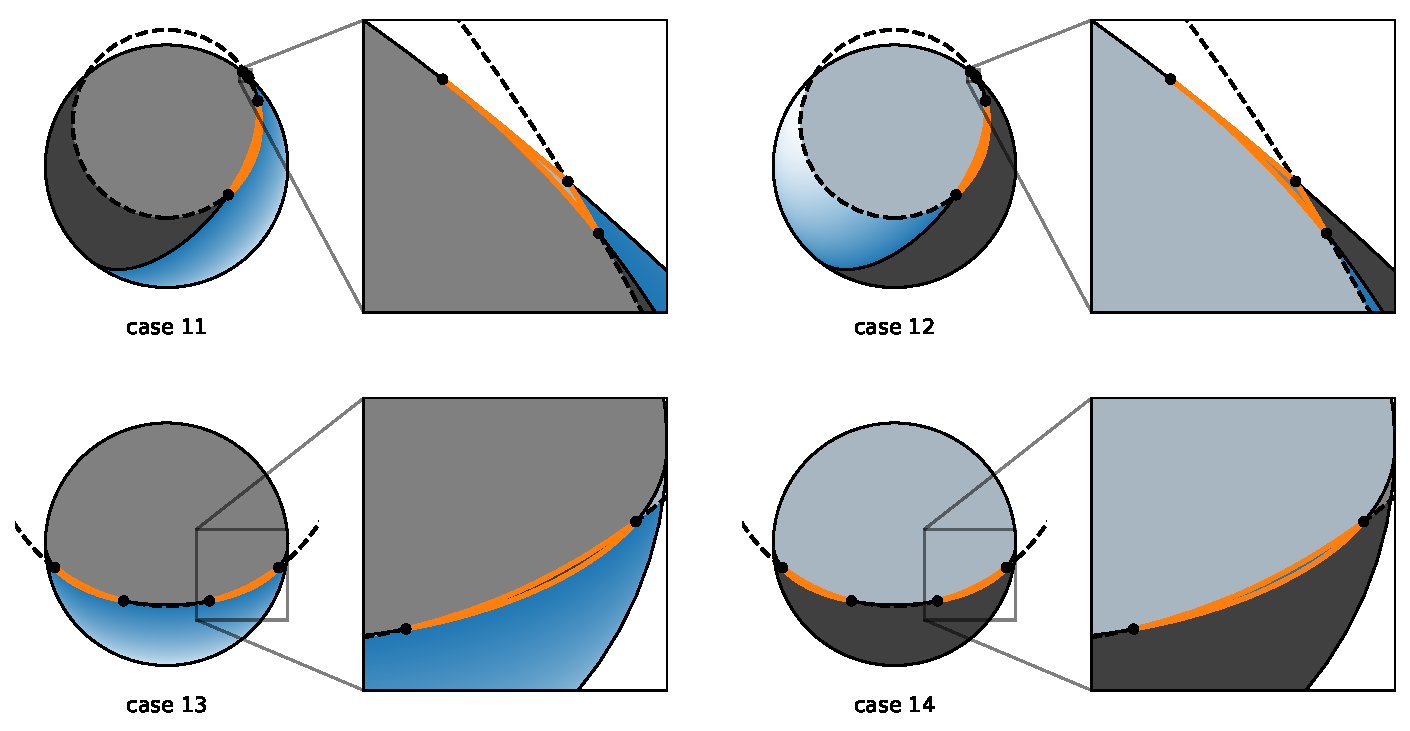
\includegraphics[width=\linewidth]{figures/pathological.pdf}
        \oscaption{pathological}{%
            Four additional families of occultations in reflected light,
            involving rare triple (cases 11 and 12, top) and quadruple
            (cases 13 and 14, bottom) intersections between the limb of the
            occultor and the terminator of the occulted body. All four cases
            involve integration over two disjoint regions (bounded by
            the orange curves in the figure). The insets next to each case
            show a zoomed-in version of four such regions. See text for
            more details.
            \label{fig:pathological}
        }
    \end{centering}
\end{figure}

Cases 11--14 correspond to (rare) configurations involving three
or four roots to Equation~\ref{eq:quartic} and are
illustrated in Figure~\ref{fig:pathological}. All four involve integration over
two disjoint regions (see the figure).
%
Cases 11 and 12 involve three points of intersection between the terminator
and the occultor limb. In case 11, the regions of integration $S_1$ and
$S_2$ are the
occulted portion of the dayside, so the solution is similar to
that of cases 6 and 8:
%
\begin{proof}{}
    \label{eq:f11}
    f_{11} = f_0 - (f_{S_1} + f_{S_2})
    \quad,
\end{proof}
%
where $f_{S_1}$ and $f_{S_2}$ are computed from Equation~(\ref{eq:fS}) for
each of the integration regions. Conversely, in case 12 the two regions
are the occulted portion of the nightside, so the solution is similar to that
of case 7:
%
\begin{proof}{}
    \label{eq:f12}
    f_{12} = f_I - \big(\hat{f}_0 - (f_{S_1} + f_{S_2})\big)
    \quad,
\end{proof}
%
Finally, cases 13 and 14 involve four points of intersection between the
terminator and the occultor limb. The regions of integration in case 13 are
the visible portion of the nightside, so this case is equivalent to case 9:
%
\begin{proof}{}
    \label{eq:f13}
    f_{13} = f_I - (f_{S_1} + f_{S_2})
    \quad.
\end{proof}
%
Conversely, the regions of integration in case 14 are the
visible portion of the dayside, so this case is equivalent to case 10:
%
\begin{proof}{}
    \label{eq:f14}
    f_{14} = f_{S_1} + f_{S_2}
    \quad.
\end{proof}
%

\subsection{Computing the integrals $\sT$}
\label{sec:sT}
%
In the previous sections, we discussed how to identify the case
corresponding to a specific configuration of the occultor and the
illumination source. We showed how in some cases
(1--5; \S\ref{sec:cases-easy}) the total flux may be
computed by exploiting the classical \starry integrals (Equation~\ref{eq:fI}).
In all other cases (6--14; \S\ref{sec:cases-hard} and
\S\ref{sec:cases-pathological}), however, the flux computation involves
evaluation of
Equation~(\ref{eq:fS}), where the solution vector $\sT$
is the vector of integrals (in the frame $\mathcal{F}'$)
of each of the terms in the Green's basis $\bg$
over a region $S$ of the
projected disk of the occultor (Equation~\ref{eq:sTint}).
%
As in \citet{Luger2019}, the approach to computing $\sT$
is to use Green's theorem to transform the surface integrals into line
integrals along the curves $\mathcal{P}$, $\mathcal{T}$, and $\mathcal{Q}$
(see Figure~\ref{fig:geometry}). Specifically, we write%
\footnote{%
    In this section, we deliberately drop the dependence of $\sT$ and
    the primitive
    integrals on the geometrical parameters $b, \theta', b_o, r_o$
    for clarity.
}
%
\begin{align}
    \label{eq:greens}
    \sT
     & =
    \iint\limits_{S}
    \bg^\top(x', y')
    \ \dd x' \ \dd y'
    \nonumber \\[0.5em]
     & =
    \oint \bvec{G}^\top (x', y') \cdot
    \dd \bvec{r} (x', y')
    \quad,
\end{align}
%
where $\bvec{G} (x', y')$
is a vector of two-dimensional Cartesian vectors chosen such that its
exterior derivative is $\bg$,
%
\begin{align}
    \label{eq:DGg}
    \frac{\dd \bvec{G}_{y'}(x', y')}{\dd x'}
    - \frac{\dd \bvec{G}_{x'}(x', y')}{\dd y'} = \bg(x', y')
    \quad,
\end{align}
%
and
%
\begin{align}
    \dd \mathbf{r} (x', y') & =
    \left(\frac{\dd x'}{\dd \varphi}\right) \dd \varphi \, \xhat' +
    \left(\frac{\dd y'}{\dd \varphi}\right) \dd \varphi \, \yhat'
    \quad,
\end{align}
%
where $\varphi$ is the parametrized angle along the integration path
and the integral is taken in a counter-clockwise direction relative to
the center of the integration region.
%
\citet{Luger2019} showed that one possible solution to
Equation~(\ref{eq:DGg}) consists of the vector whose $n^\text{th}$
component is given by
%
\begin{align}
    \label{eq:G}
    \mathbf{G}_n (x', y') & =
    \begin{dcases}
        %
        x'^{\frac{\mu + 2}{2}}
        y'^{\frac{\nu}{2}}
        \,\yhat'
         & \qquad \mu, \nu \, \text{even}
        \\[1em]
        %
        \frac{1-z(x', y')^3}{3(1-z(x', y')^2)}\bigg(-y' \, \xhat' + x' \, \yhat'\bigg)
         & \qquad \mu = \nu = 1
        \\[1em]
        %
        x'^{l-2}
        z(x', y')^3
        \,\xhat
         & \qquad \nu \, \text{odd}, \,
        \mu = 1, \,
        l \, \text{even}
        \\[1em]
        %
        x'^{l-3}
        y'
        z(x', y')^3
        \,\xhat
         & \qquad \nu \, \text{odd}, \,
        \mu = 1, \,
        l \, \text{odd}
        \\[1em]
        %
        x'^{\frac{\mu-3}{2}}
        y'^{\frac{\nu-1}{2}}
        z(x', y')^3
        \,\yhat
         & \qquad \text{otherwise,}
    \end{dcases}
\end{align}
%
where the indices $l, m, \mu, \nu$ are given by
Equations~(\ref{eq:l-m}) and (\ref{eq:mu-nu}).

We showed in the previous sections that there are at most three curves
$\mathcal{P}$, $\mathcal{T}$, and $\mathcal{Q}$ bounding a given closed surface of integration
(see Figure~\ref{fig:geometry}). We may therefore express
Equation~(\ref{eq:greens}) as
%
\begin{proof}{}
    \label{eq:sT}
    \sT & =
    \pT + \tT + \qT
    \quad,
\end{proof}
%
where we define the primitive integrals%
\footnote{%
    The components of the vectors $\pT$ and
    $\qT$ are analogous to the primitive integrals
    $\mathcal{P}$ and $\mathcal{Q}$
    defined in Equations~(30)--(32) in \citet{Luger2019}, although the
    integration limits of both and the sense of integration of $\mathcal{P}$
    are different.
}
%
\begin{proof}{}
    \label{eq:pT}
    \pT
    & =
    \int\limits_{\pmb{\phi}}
    \mathbf{G}^\top(x'_p, y'_p)
    \cdot \dd \mathbf{r}(x'_p, y'_p)
    %
    \\
    %
    \label{eq:tT}
    \tT
    & =
    \int\limits_{\pmb{\xi}}
    \mathbf{G}^\top(x'_t, y'_t)
    \cdot \dd \mathbf{r}(x'_t, y'_t)
    %
    \\
    %
    \label{eq:qT}
    \qT
    & =
    \int\limits_{\pmb{\lambda}}
    \mathbf{G}^\top(x'_q, y'_q)
    \cdot \dd \mathbf{r}(x'_q, y'_q)
\end{proof}
%
to be the line integrals of $\mathbf{G}$ along each of the curves
$\mathcal{P}$, $\mathcal{T}$, and $\mathcal{Q}$, respectively, where the coordinates along each
curve are parametrized
in terms of $\varphi$ as follows:
%
\\[1em]
%
\begin{minipage}{0.3\linewidth}
    \begin{align}
        x'_p & = r_o \cos\varphi
        \nonumber                      \\
        y'_p & = b_o + r_o \sin\varphi
        \nonumber
    \end{align}
\end{minipage}
%
\begin{minipage}{0.34\linewidth}
    \begin{align}
        x'_t & = \cos\theta' \cos\varphi - b \sin\theta' \sin\varphi
        \nonumber                                                    \\
        y'_t & = \sin\theta' \cos\varphi + b \cos\theta' \sin\varphi
        \nonumber
    \end{align}
\end{minipage}
%
\begin{minipage}{0.3\linewidth}
    \begin{proof}{}
        \label{eq:xy_pqt}
        x'_q & =\cos\varphi
        \nonumber           \\
        y'_q & = \sin\varphi
        \quad,
    \end{proof}
\end{minipage}
%
\\[1em]
%
and we define
%
\begin{align}
    \label{eq:vint}
    \int\limits_{\pmb{\varphi}} & \equiv
    %
    \int\limits_{\varphi_{0}}^{\varphi_{1}}
    +
    \int\limits_{\varphi_{2}}^{\varphi_{3}}
    +
    \cdots
    +
    \int\limits_{\varphi_{N - 2}}^{\varphi_{N - 1}}
    %
    \nonumber                            \\
                                & \equiv
    \sum_{i = 0}^{\frac{N - 1}{2}}
    \int\limits_{\varphi_{2i}}^{\varphi_{2i+1}}
\end{align}
%
to be the sum of definite integrals between pairs of limits $\varphi_i$
arranged in a vector $\pmb{\varphi}$ of length $N$.
%
For future reference, it will also be useful to define the operator
%
\begin{align}
    \label{eq:pairdiff}
    \Delta \mathbf{x} \equiv \sum_{i=0}^{\frac{N - 1}{2}}
    \left( x_{2i + 1} - x_{2i} \right)
    \quad,
\end{align}
%
which sums the difference of successive pairs of values in
a vector
$\mathbf{x} = \left( x_0, x_1, x_2, x_3, {\cdot\cdot\cdot}, x_{N - 1} \right)^\top$.
This will come in handy when computing definite integrals. Specifically,
if $g$ is the antiderivative of some function $f$, we may use the
fundamental theorem of calculus to compute the integral of
$f$ over the interval(s) given
by the vector of limit pairs $\pmb{\varphi}$:
%
\begin{align}
    \vint{\pmb{\varphi}}{f(\varphi)}
     & = \int\limits_{\varphi_{0}}^{\varphi_{1}} f(\varphi) \dd\varphi
    +
    \int\limits_{\varphi_{2}}^{\varphi_{3}} f(\varphi) \dd\varphi
    +
    {\cdot\cdot\cdot}
    +
    \int\limits_{\varphi_{N - 2}}^{\varphi_{N - 1}} f(\varphi) \dd\varphi
    \nonumber                                                          \\
     & = \Delta \mathbf{g}(\pmb{\varphi})
\end{align}
%
where $\mathbf{g}$ is the vector given by
%
\begin{align}
    \mathbf{g}(\pmb{\varphi}) =
    \bigg( g(\varphi_0), g(\varphi_1), g(\varphi_2), g(\varphi_3),
    {\cdot\cdot\cdot}, g(\varphi_{N - 2}), g(\varphi_{N - 1}) \bigg)^\top
    \quad.
\end{align}
%
Note that most of the cases (1--10) involve integration over a single closed
region, so Equations~(\ref{eq:vint}) and (\ref{eq:pairdiff}) reduce to
%
\begin{align}
    \int\limits_{\pmb{\varphi}} & \equiv
    %
    \int\limits_{\varphi_{0}}^{\varphi_{1}}
\end{align}
%
and
%
\begin{align}
    \Delta \mathbf{x} \equiv x_1 - x_0
    \quad.
\end{align}
%
For cases 11--14, we must integrate over two disjoint regions, so we
sum over two pairs of limits.
%
In the next three sections, we derive the solutions to each of the
primitive integrals $\pT$, $\tT$, and $\qT$.

\subsection{The integral along the occultor limb, $\pT$}
\label{sec:pT}
%
In this section we present a solution to Equation~(\ref{eq:pT}). The first
order of business is to derive expressions for the integration limits
$\pmb{\phi}$. Depending on the integration case, these limits will correspond
to the point of intersection between the limb of the occultor and the
limb of the occulted body and/or the point of intersection between the limb
of the occultor and the terminator of the occulted body.
The former is given by
\citep[c.f. Equation~24 in][]{Luger2019}
%
\begin{align}
    \phi_0 & =
    \frac{\pi}{2} \pm \left(\arcsin\left(\frac{1 - r_o ^ 2 - b_o ^ 2}{2 b_o r_o}\right) - \frac{\pi}{2}\right)
    \quad,
\end{align}
%
where the sign is chosen such that the point
$(r_o\cos\phi_0, b_o + r_o\sin\phi_0)$ is on the dayside of the occulted body,
and the latter (of which there may be multiple) is given by
%
% Introduce the function
% %
% \begin{proof}{}
%     \textrm{\faAdjust}(x, y) &=
%     \begin{cases}
%         \textrm{\faCircleO} & \qquad -x \sin\theta' + y\cos\theta' \ge b \sqrt{1 - (x\cos\theta' + y\sin\theta') ^ 2}
%         \\
%         \textrm{\faCircle}  & \qquad \text{otherwise}
%     \end{cases}
% \end{proof}
% %
% which returns \faCircleO\ if point $(x, y)$ is on the dayside of the body and
% \faCircle\ if it is on the nightside.
%
%
\begin{align}
    \pmb{\phi_1} & =
    \theta' +
    \atantwo
    \left(b\sqrt{1 - {\mathbf{x''}}^2 - y''_o}, \mathbf{x''} - x''_o\right)
    \quad
\end{align}
%
where $\mathbf{x''}$ are the roots of the quartic (Equation~\ref{eq:quartic}).
These angles are then wrapped to the range $[0, 2\pi)$
and sorted into the vector $\pmb{\phi}$ such that
the integration is always performed in a counter-clockwise sense about
the center of the integration region.
%
The left panel in Figure~\ref{fig:geometry} shows a configuration in which
the lower integration limit $\phi_0 = 158.2^\circ$ corresponds to the
point of intersection between the limbs of the two bodies and the upper
integration limit $\phi_1 = 223.3^\circ$ corresponds to the
limb-terminator intersection. Both angles are measured counter-clockwise
from the line $x' = b_o$.

In order to evaluate the integral in Equation~(\ref{eq:pT}),
we follow the reparametrization tricks of \S{D.2.3} in \citet{Luger2019}.
The algebra is long and tedious, so we merely present the result
(alongside the usual validation links). The $n^\text{th}$ component
of $\pT$ is
%
\begin{proof}{}
    \label{eq:pTsoln}
    \mathbb{p}_n & =
    \resizebox{.8\hsize}{!}{$
            \begin{cases}
                %
                2(2r_o)^{l+2}
                %
                \begin{cases}
                    %
                    V
                    \left(
                    \frac{\mu+4}{4},
                    \frac{\nu}{2},
                    0;
                    \viI
                    \right)
                    %
                     & \qquad \qquad \qquad \qquad \qquad
                    \qquad \qquad \qquad \quad
                    \frac{\mu}{2} \, \text{even}
                    \\[0.5em]
                    %    
                    V
                    \left(
                    \frac{\mu + 2}{2},
                    \frac{\nu}{2},
                    0;
                    \viU
                    \right)
                    %
                     & \qquad \qquad \qquad \qquad \qquad
                    \qquad \qquad \qquad \quad
                    \frac{\mu}{2} \, \text{odd}
                    %
                \end{cases}
                %
                 & \qquad
                \mu, \nu \, \text{even}
                %
                \\[2em]
                %
                \mathbb{p}_2
                %
                 & \qquad
                \mu = \nu = 1
                %
                \\[1.5em]
                %
                \beta (2r_o)^{l-1}
                %
                \begin{cases}
                    %
                    \begin{cases}
                        %
                        V
                        \left(
                        \frac{l-2}{2},
                        0,
                        0;
                        \viJ
                        \right) -
                        2
                        V
                        \left(
                        \frac{l-2}{2},
                        0,
                        1;
                        \viJ
                        \right)
                        %
                         & \qquad \quad
                        l \, \text{even}
                        %
                        \\[1em]
                        %
                        V
                        \left(
                        \frac{l-3}{2},
                        1,
                        0;
                        \viJ
                        \right) -
                        2V
                        \left(
                        \frac{l-3}{2},
                        1,
                        1;
                        \viJ
                        \right)
                        %
                         & \qquad \quad
                        l \, \text{odd} \ne 1
                        %
                    \end{cases}
                    %
                     & \qquad
                    \mu = 1
                    %
                    \\[3em]
                    %
                    \begin{cases}
                        %
                        2
                        V
                        \left(
                        \frac{\mu-1}{4},
                        \frac{\nu-1}{2},
                        0;
                        \viJ
                        \right)
                        %
                         & \qquad \qquad \qquad \qquad
                        \frac{\mu - 1}{2} \, \text{even}
                        %
                        \\[1em]
                        %
                        2
                        V
                        \left(
                        \frac{\mu-1}{4},
                        \frac{\nu-1}{2},
                        0;
                        \viW
                        \right)
                        %
                         & \qquad \qquad \qquad \qquad
                        \frac{\mu - 1}{2} \, \text{odd}
                        %
                    \end{cases}
                    %
                     & \qquad
                    \mu > 1
                    %
                \end{cases}
                %
                 & \qquad
                \mu, \nu \, \text{odd}
                %
            \end{cases}
        $}
\end{proof}
%
where $\beta = \left(1 - (b_o - r_o)^2\right)^\frac{3}{2}$
and we define the Vieta operator
%
\begin{align}
    \label{eq:V}
    V\left(u, v, w; \mathbf{x}\right) \equiv
    \sum_{i=0}^{u + v}
    \mathcal{A}_{u, v, i}
    \mathbf{x}_{u + w + i}
\end{align}
%
as the dot product of a vector $\mathbf{x}$ and
the vector of Vieta's theorem coefficients, where
\citep[c.f. Equation~D34 in][]{Luger2019}
%
\begin{align}
    \label{eq:vieta}
    \mathcal{A}_{u,v,i} & =
    \sum_{j=\text{max}(0,u-i)}^{\text{min}(u+v-i,u)}
    \binom{u}{j}
    \binom{v}{u+v-i-j}
    (-1)^{u+j}\left(\frac{b_o-r_o}{2r_o}\right)^{u+v-i-j}
    \quad.
\end{align}
%
The vectors $\viI$, $\viJ$,
$\viU$, and $\viW$ are solutions
to specific integrals, which we compute recursively below. As in
\citet{Luger2019} the $n = 2$ term of $\pT$, $\mathbb{p}_2$,
is handled separately; we also compute this below.

Note that several of the cases in Equation~(\ref{eq:pTsoln}) are
identical to those in Equation~(D35) of \citet{Luger2019}, provided
we replace their integrals $\mathcal{I}$ and $\mathcal{J}$ with our
integrals $\viI$ and $\viJ$, respectively. The integrals themselves
are similar, except for a change in the limits of integration, which
are no longer symmetric about zero. As we will see, this leads to the
dependence of these expressions on \emph{incomplete} elliptic integrals.
Note also that the integrals $\viU$ and $\viW$ are new, as certain
cancellations in \citet{Luger2019} resulted in the corresponding cases
contributing zero net flux \citep[last case in Equation~D35 of][]{Luger2019}.

%

\subsubsection{The vector $\viI$}
\label{sec:I}
%
The components of the vector $\viI$ are given by the integral
%
\begin{align}
    \label{eq:I}
    \iI_v(\valpha) & =
    \vint{\valpha}{\sin^{2v}\varphi}
    \quad,
\end{align}
%
for $v \in [0, \vmax]$,
where we define the helper angle
%
\begin{align}
    \label{eq:alpha}
    \valpha \equiv \frac{\pmb{\phi}}{2} + \frac{\pi}{4}
    \quad.
\end{align}
%
The integral in the expression above is the same as that in Equation (D38)
of \citet{Luger2019}, except for a change in the limits of integration.
As in \citet{Luger2019}, we can compute the vector $\viI$ recursively given
a trivial lower boundary condition:
%
\begin{proof}{I}
    \label{eq:Irec}
    \iI_0(\valpha) &=
    \Delta \valpha
    %
    \nonumber \\
    %
    \iI_v(\valpha) &=
    \frac{1}{2v}
    \bigg(
    (2v - 1) \iI_{v-1}(\valpha) -
    \Delta \left(\sin^{2v - 1}\valpha\cos^{2v -1}\valpha\right)
    \bigg)
\end{proof}
%
where the last expression is valid for all $v > 0$. We find that this algorithm
is generally stable, except when
$\sin\valpha$ is small.
In that limit, we evaluate $\iI_\vmax(\valpha)$
by numerical integration of
Equation~(\ref{eq:I}) using Gauss-Legendre quadrature with \STARRYQUADPOINTS
points. We then recurse downward by substituting $v \rightarrow v + 1$ in
Equation~(\ref{eq:Irec}) and solving for $\iI_v(\valpha)$.

%

\subsubsection{The vector $\viJ$}
\label{sec:J}
%
The components of the vector $\viJ$ are given by the integral
%
\begin{align}
    \label{eq:J}
    \iJ_v(k^2, \valpha) =
    \vint{\valpha}{
        \sin^{2v}\varphi
        \left(1 - \frac{\sin^2\varphi}{k^2}\right)^\frac{3}{2}
    }
    \quad,
\end{align}
%
where
%
\begin{align}
    \label{eq:k2}
    k^2 & \equiv \frac{1 - r_o^2 - b_o^2 + 2 b_o r_o}{4 b_o r_o}
    \quad.
\end{align}
%
The integral in this expression is again the same as that in Equation (D39)
of \citet{Luger2019}, except for a change in the limits of integration.
In that paper, we computed all terms
$\{ \iJ_0, {\cdot\cdot\cdot}, \iJ_\vmax \}$ from a three-term
recurrence relation and two boundary conditions. In the case of upward
recursion, the boundary conditions $\iJ_0$ and $\iJ_1$ were
computed analytically from the complete elliptic integrals $K(k^2)$
and $E(k^2)$. In cases where upward recursion was not numerically stable, we
evaluated $\iJ_\vmax$ and $\iJ_{\vmax-1}$
via a quickly convergent series expansion and recursed downward.

In order to solve Equation~(\ref{eq:J}), it is possible to
replace the complete elliptic integrals $K(k^2)$ and $E(k^2)$ in the lower
boundary conditions \citep[Equation D46 in ][]{Luger2019} with the
incomplete elliptic integrals
%
\begin{align}
    \label{eq:F}
    F(\psi \,|\, m) & \equiv \int_0^{\psi} \frac{\dd \varphi}{\sqrt{1 - m \sin^2 \varphi}}
    \\
    \intertext{and}
    \label{eq:E}
    E(\psi \,|\, m) & \equiv \int_0^{\psi} \sqrt{1 - m \sin^2 \varphi} \, \dd \varphi
    \quad,
\end{align}
%
which we compute from the $el\mathit{2}$ parametrization of
\citet{Bulirsch1965},
%
then use the same upward
recursion relation to obtain analytic solutions for all $\iJ_v$:
%
\begin{proof}{J}
    \label{eq:Jrec}
    \iJ_0(k^2, \valpha) &=
    \frac{1}{3} \bigg(
    2 \left(2 - \frac{1}{k^2}\right) \DE +
    \left(\frac{1}{k^2} - 1\right) \DF +
    \Delta \mathbf{z}_0(k^2, \valpha)
    \bigg)
    %
    \nonumber \\
    %
    \iJ_1(k^2, \valpha) &=
    \frac{1}{15} \bigg(
    \left(-3 k^2 + 13 - \frac{8}{k^2}\right) \DE
    \nonumber \\
    &\qquad\quad\quad\quad\quad\quad\quad\quad\quad
    +
    \left(3 k^2 - 7 + \frac{4}{k^2}\right) \DF +
    \Delta \mathbf{z}_1(k^2, \valpha)
    \bigg)
    %
    \nonumber \\
    %
    \iJ_v(k^2, \valpha) &=
    \frac{1}{2v + 3}
    \bigg(
    2 \left( v + 1 + (v - 1) k^2 \right) \iJ_{v - 1}(k^2, \valpha)
    \nonumber \\
    &\qquad\qquad\quad\quad\quad\quad
    -
    (2v - 3) k^2 \iJ_{v - 2}(k^2, \valpha)
    + \Delta \mathbf{z}_v(k^2, \valpha)
    \bigg)
\end{proof}
%
%
where the last expression is valid for all $v > 1$ and
%
\begin{proof}{J}
    \label{eq:Jrec_z}
    \mathbf{z}_0(k^2, \valpha) & =
    \frac{
        \sin\valpha
        \cos\valpha
        \,
        \mathbf{q}(k^2, \valpha)
    }{
        k^2
    }
    %
    \nonumber\\
    %
    \mathbf{z}_1(k^2, \valpha) & =
    \left(3 \sin^2\valpha + 4 - 6k^2\right)
    \mathbf{z}_0(k^2, \valpha)
    %
    \nonumber\\
    %
    \mathbf{z}_v(k^2, \valpha) & =
    k^2
    \sin^{2v - 3}\valpha
    \cos\valpha
    \,
    \mathbf{q}(k^2, \valpha)^5
    \quad,
\end{proof}
%
with
%
\begin{align}
    \label{eq:q}
    \mathbf{q}(k^2, \valpha) = \sqrt{1 - \frac{\sin^2\valpha}{k^2}}
    \quad.
\end{align}
%
Note that when $k^2 < 1$ we use the reciprocal-modulus transformation
to evaluate the elliptic integrals:
%
\begin{align}
    F\left(\psi \,\Big|\, \frac{1}{k^2}\right) & =
    k \, F(\beta \,|\, k^2)
    \nonumber                                                                               \\
    E\left(\psi \,\Big|\, \frac{1}{k^2}\right) & =
    \frac{E(\beta \,|\, k^2) - (1 - k^2) F(\beta \,|\, k^2)}{k}
    \\
    \intertext{with}
    \beta                                      & = \arcsin\left( \frac{\sin\psi}{k} \right)
    \quad.
\end{align}
%

In practice, however, we find that this procedure is even more numerically
unstable than it was in \citet{Luger2019}.
To address this, we express the recurrence structure of the problem as
a tridiagonal system with one lower boundary condition $\iJ_0$
and one upper boundary condition $\iJ_\vmax$:
%
\begin{proof}{J}
    \label{eq:Jtri}
    \begin{pmatrix}
        a_0 & 1   &     &        &         &         \\
        b_1 & a_1 & 1   &        &         &         \\
            & b_2 & a_2 & 1      &         &         \\
            &     & b_0 & a_3    & 1       &         \\
            &     &     & \ddots & \ddots  & \ddots  \\
            &     &     &        & b_\vmax & a_\vmax
    \end{pmatrix}
    \begin{pmatrix}
        \iJ_1           \\
        \iJ_2           \\
        \iJ_3           \\
        \iJ_4           \\
        \cdot\cdot\cdot \\
        \iJ_{\vmax-1}
    \end{pmatrix}
    =
    \begin{pmatrix}
        c_0 - b_0 \iJ_0 \\
        c_1             \\
        c_2             \\
        c_3             \\
        \cdot\cdot\cdot \\
        c_\vmax - \iJ_\vmax
    \end{pmatrix}
\end{proof}
%
where the recursion coefficients are given by
%
\begin{proof}{J}
    \label{eq:Jtri_coeffs}
    a_v(k) &= -2\frac{(v + 1) + (v - 1) k^2}{2v + 3} \nonumber \\
    b_v(k) &= \frac{(2v - 3) k^2}{2v + 3} \nonumber \\
    c_v(k^2, \valpha) &= \Delta
    \bigg(
    \frac{
            \mathbf{z}_v(k^2, \valpha)
        }{
            2v + 3
        }
    \bigg)
    \quad.
\end{proof}
%
Solving this matrix system yields values for all
intermediate $\{ \iJ_1, {\cdot\cdot\cdot}, \iJ_{\vmax - 1} \}$.
While efficient algorithms exist for solving tridiagonal problems, we obtain
far better numerical stability by instead performing traditional LU
decomposition. We find that this algorithm is stable in all the regimes that we
tested.

We evaluate the upper boundary condition $\iJ_{\vmax}$ by numerical
integration of Equation~(\ref{eq:J}) via Gauss-Legendre quadrature with
\STARRYQUADPOINTS points. While the lower boundary condition may be computed
analytically from Equation~(\ref{eq:Jrec}),
in practice we achieve better precision via numerical
integration (as above), with negligible effects on computational performance.

%

\subsubsection{The vector $\viU$}
\label{sec:U}
%
The components of the vector $\viU$ are given by the integral
%
\begin{align}
    \label{eq:U}
    \iU_v(\valpha) =
    \vint{\valpha}{\cos\varphi\sin^{2v + 1}\varphi}
    \quad.
\end{align}
%
This integral has an analytic solution for all $v$:
%
\begin{proof}{U}
    \label{eq:Usol}
    \iU_v(\valpha) &= \frac{\Delta \sin^{2v+2}\valpha}{2v + 2}
    \quad.
\end{proof}
%

\subsubsection{The vector $\viW$}
\label{sec:W}
%
The components of the vector $\viW$ are given by the integral
%
\begin{align}
    \label{eq:W}
    \iW_v(k^2, \valpha) =
    \vint{\valpha}{
        \cos\varphi\sin^{2v + 1}\varphi
        \left(1 - \frac{\sin^2\varphi}{k^2}\right)^\frac{3}{2}
    }
    \quad.
\end{align}
%
We may compute it by either upward or downward recursion. In both cases,
we compute each of the $\iW_v$ from
%
\begin{proof}{W}
    \iW_v(k^2, \valpha) = \Delta \mathbf{b}_v(k^2, \valpha)
    \quad.
\end{proof}
%
In the upward case, we start with the lower boundary conditions
%
\begin{proof}{W}
    \mathbf{b}_0(k^2, \valpha) &=
    \frac{\sin^2\valpha}{5}
    \left(
    \frac{1 - \mathbf{q}(k^2, \valpha)^3}{1 - \mathbf{q}(k^2, \valpha)^2}
    +
    \mathbf{q}(k^2, \valpha)^3
    \right)
    \nonumber \\
    \mathbf{c}_0(k^2, \valpha) & =
    \sin^4\valpha \,
    \frac{\mathbf{q}(k^2, \valpha)^5}{1 - \mathbf{q}(k^2, \valpha)^2}
    \quad,
\end{proof}
%
and recurse upward in $\mathbf{b}$ and $\mathbf{c}$ simultaneously:
%
\begin{proof}{W}
    \mathbf{b}_v(k^2, \valpha) & =
    \frac{1}{2v + 5}
    \left(
    \frac{2 v \sin^2\valpha}{1 - \mathbf{q}(k^2, \valpha)^2}
    \mathbf{b}_{v - 1}(k^2, \valpha)
    - \mathbf{c}_{v - 1}(k^2, \valpha)
    \right)
    \nonumber
    \\
    \mathbf{c}_v(k^2, \valpha) & =
    \sin^2\valpha \, \mathbf{c}_{v - 1}(k^2, \valpha)
\end{proof}
%
for $v > 0$.
%
In the case of downward recursion, we start with the upper boundary
conditions
%
\begin{proof}{W}
    \mathbf{b}_\vmax &=
    \frac{\sin^{2\vmax + 2}\valpha}{4\vmax + 10}
    \left(
    \mathbf{f}_\vmax(k^2, \valpha)
    + 2 \mathbf{q}(k^2, \valpha)^3
    \right)
    \nonumber \\
    \mathbf{c}_\vmax &=
    \frac{1}{2}
    \mathbf{q}(k^2, \valpha)^5
    \sin^{2\vmax}\valpha
    \quad,
\end{proof}
%
where
%
\begin{proof}{W}
    \mathbf{f}_v(k^2, \valpha)
    &\equiv
    \frac{3}{v+1}
    \,
    {_2\pmb{F}_1}\left(
    -\frac{1}{2},
    v + 1;
    v + 2;
    1 - \mathbf{q}(k^2, \valpha)^2
    \right)
\end{proof}
%
and ${_2\pmb{F}_1}(a, b; c; \mathbf{z})$ is the Gauss
hypergeometric function, which we compute via its series
definition.
%
We recurse downward in $\mathbf{b}$ and $\mathbf{c}$ simultaneously:
%
\begin{proof}{W}
    \mathbf{b}_v(k^2, \valpha) & =
    \frac{1 - \mathbf{q}(k^2, \valpha)^2}{\sin^2\valpha}
    \left(1 + \frac{5}{2v + 2}\right)
    \mathbf{b}_{v + 1}(k^2, \valpha) +
    \frac{\mathbf{c}_{v + 1}(k^2, \valpha)}{v + 1}
    \nonumber
    \\
    \mathbf{c}_v(k^2, \valpha) & =
    \frac{\mathbf{c}_{v + 1}(k^2, \valpha)}{\sin^2\valpha}
    \quad.
\end{proof}

%

\subsection{The term $\mathbb{p}_2$}
\label{sec:p2}
%
The final integral we must solve is that corresponding to
$\mathbb{p}_2$ ($\mu = \nu = 1$). As in \citet{Luger2019}, this is
the integral of the linear limb darkening term,
whose solution must be handled
separately due to the fact that the corresponding antiderivative
in Equation~(\ref{eq:G}) is not a polynomial in $x$, $y$, and $z(x, y)$.
The integral we must solve is
%
\begin{align}
    \label{eq:p2}
    \mathbb{p}_2 & =
    \vint{\pmb{\phi}}{
        \frac{1}{3}
        \left(
        \frac{
            1 - z(r_o\cos\varphi, b_o + r_o\sin\varphi)^3
        }{
            1 - z(r_o\cos\varphi, b_o + r_o\sin\varphi)^2
        }
        \right)
        \left(r_o^2 + b_o r_o \sin\varphi\right)
    }
    \quad,
\end{align}
%
where $z$ is the usual Cartesian coordinate (Equation~\ref{eq:z}).
The solution is tricky, but fortunately a similar integral was solved in
Equation~(34) of \citet{Pal2012}. Adapting their solution to our formalism,
we obtain
%
\begin{proof}{p2}
    \label{eq:p2_soln}
    \mathbb{p}_2 & =
    \frac{1}{3}
    \Big(
    c_0 +
    c_1 \DF +
    c_2 \DE +
    c_3 \DPi
    \Big)
\end{proof}
%
where
%
\begin{proof}{p2}
    c_0 &=
    \Delta
    \Bigg\{
    -\atantwo\left(
    -(b_o - r_o) \cos\valpha, (b_o + r_o) \sin\valpha
    \right)
    + \valpha
    \nonumber \\
    &\qquad\enspace\enspace
    - \frac{4}{3} b_o r_o
    \sin\valpha \cos\valpha
    \sqrt{1 - (b_o - r_o)^2 - 4 b_o r_o \sin^2\alpha}
    \nonumber \\
    &\qquad\enspace\enspace
    + \pmb{\delta}(b_o, r_o, \valpha)
    \Bigg\}
    \nonumber \\[0.5em]
    c_1 &=
    \frac{1 + b_o^4 - b_o^2(5 + 2 r_o^2) + r_o^4 + r_o^2}{3 \sqrt{1 - (b_o - r_o)^2}}
    \nonumber \\[0.5em]
    c_2 &= \frac{(b_o^2+7r_o^2-4)\sqrt{1 - (b_o - r_o)^2}}{3}
    \nonumber \\[0.5em]
    c_3 &= \frac{b_o + r_o}{(b_o - r_o)\sqrt{1 - (b_o - r_o)^2}}
    \quad,
    \\
    \intertext{and}
    %
    \delta(b_o, r_o, \alpha) &=
    \begin{cases}
        -2\pi
         &
        \qquad
        \alpha > \frac{3\pi}{2} \,\, \text{and} \,\, b_o > r_o
        \\
        +2\pi
         &
        \qquad
        \alpha > \frac{3\pi}{2} \,\, \text{and} \,\, b_o < r_o
        \\
        0
         &
        \qquad
        \text{otherwise}
        \quad.
    \end{cases}
\end{proof}
%
The quantities $\pmb{F}(\valpha \,|\, \nicefrac{1}{k^2})$ and
$\pmb{E}(\valpha \,|\, \nicefrac{1}{k^2})$
are the same incomplete elliptic integrals as those in
\S\ref{sec:J}, while
%
\begin{align}
    \label{eq:Pi}
    \Pi(n; \psi \,|\, m) & \equiv
    \int_0^{\psi}
    \frac{\dd \varphi}{(1 - n \sin^2\varphi)\sqrt{1 - m \sin^2 \varphi}}
\end{align}
%
is the incomplete elliptic integral of the third
kind, with
%
\begin{proof}{p2}
    \label{eq:n}
    n & = -\frac{4 b_o r_o}{(r_o - b_o)^2}
    \quad.
\end{proof}
%

While stable algorithms exist to evaluate $\Pi(n; \psi \,|\, m)$
\citep[e.g.][]{Bulirsch1969}, we find that the parametrization above has
poor numerical stability, particularly in the vicinity of the singular
points $b_o = r_o$ and $b_o = 1 + r_o$. In practice, we find that
numerical evaluation of Equation~(\ref{eq:p2}) via Gaussian quadrature
is more numerically stable and just as computationally efficient as
the procedure outlined above.

\subsection{The integral along the terminator, $\tT$}
\label{sec:tT}
%
In this section we present a solution to Equation~(\ref{eq:tT}), the
line integral along the day/night terminator of the occulted body. As
before, the first thing we must do is derive expressions for the integration
limits $\pmb{\xi}$.
%
Depending on the integration case, these limits
will corresponds to the point of intersection between the terminator and
the limb of the occultor and/or the point of intersection between the
terminator and the limb of the occulted body. The former is given by
%
\begin{proof}{}
    \pmb{\xi_0} &=
    \atantwo\left(\sqrt{1 - {\mathbf{x''}}^2}, \mathbf{x''} \right)
\end{proof}
%
where $\mathbf{x''}$ are the roots of the quartic (Equation~\ref{eq:quartic}).
The latter is given by
%
\begin{proof}{}
    \xi_1 &=
    \begin{cases}
        0   & \qquad \qquad (1 - x_o'')^2 + {y_o''}^2 < r_o^2
        \\
        \pi & \qquad \qquad \text{otherwise}
        \quad.
    \end{cases}
\end{proof}
%
As before, these angles are then
wrapped to the range $[0, 2\pi)$ and
sorted into the vector
$\pmb{\xi}$ such that the integration is performed counter-clockwise
about the center of the integration region.
%
The middle panel of Figure~\ref{fig:geometry} shows a case where
$\xi_0 = 96.5^\circ$ corresponds to the point of intersection between the occultor
limb and the terminator and $\xi_1 = 0^\circ$ corresponds to the
point where the terminator extends onto the backside of the body.
%
Note, importantly, that unlike $\pmb{\phi}$, the angle $\pmb{\xi}$ is not
measured between the horizontal and a point on the curve of $\mathcal{T}$.
Recall that $\pmb{\xi}$ is an angular parameter of the ellipse, so it is
measured in the same way as the eccentric anomaly in a Keplerian orbit:
it is the
angle between the semi-major axis of the ellipse and the perpendicular
projection of a point on the ellipse onto the unit circle
(see Figure~\ref{fig:geometry}).

The solution to Equation~(\ref{eq:tT}) involves repeated application
of the binomial theorem. As before, we simply present the result, with
validation links:
%
\begin{proof}{}
    \mathbb{t}_n & =
    \begin{cases}
        %
        %
        b\cos\theta'
        \sum\limits_{j=0}^{\frac{\nu}{2}}
        \sum\limits_{k=0}^{\frac{\mu + 2}{2}}
        Z^{\frac{\nu}{2}, \frac{\mu+2}{2}}_{j,k}
        (b, \theta') \,
        \iH_{j + k + 1, l + 1 - j - k}(\pmb{\xi})
        \\
        \quad\quad\quad\quad
        - \, \sin\theta'
        \sum\limits_{j=0}^{\frac{\nu}{2}}
        \sum\limits_{k=0}^{\frac{\mu + 2}{2}}
        Z^{\frac{\nu}{2}, \frac{\mu+2}{2}}_{j,k}
        (b, \theta') \,
        \iH_{j + k, l + 2 - j - k}(\pmb{\xi})
        %
         & \qquad
        \mathrel{\raisebox{1.25em}{$\mu, \nu, \, \text{even}$}}
        %
        %
        \\[3em]
        %
        %
        \frac{1}{3}
        \Delta
        \Big\{
        \arctan\left( \frac{|b|\sin\vxi}{\cos\vxi} \right)
        \\
        \qquad\quad\quad
        - \, \sgn\left({\sin\vxi}\right)
        \left(
        \arctan
        \left(
            \frac{
                \left(\frac{\sin\vxi}{1 + \cos\vxi}\right)^2 + 2 b^2 - 1
            }{2 |b| b_c}
            \right)
        + |b| b_c \cos\vxi
        \right)
        %
         & \qquad \mu = \nu = 1
        %
        \\
        \qquad\quad\quad
        + \, \pmb{\delta}(b, \vxi)
        \Big\}
        %
        \\[3em]
        %
        %
        -b\sin\theta'
        \sum\limits_{j=0}^{l-2}
        Z^{0, l-2}_{0,k}
        (b, \theta') \,
        \iH_{j + 1, l + 1 - j}(\pmb{\xi})
        \\
        \quad\quad\quad\quad
        - \, \cos\theta'
        \sum\limits_{j=0}^{l-2}
        Z^{0, l-2}_{0,k}
        (b, \theta') \,
        \iH_{j, l + 2 - j}(\pmb{\xi})
        %
         & \qquad
        \mathrel{\raisebox{1.25em}{$\nu \, \text{odd}, \mu = 1, l \, \text{even}$}}
        %
        %
        \\[3em]
        %
        %
        -b\sin\theta'
        \sum\limits_{j=0}^{l-3}
        \bigg(
        \sin\theta'
        Z^{0, l-3}_{0,k}
        (b, \theta') \,
        \iH_{j + 2, l - j}(\pmb{\xi})
        \\
        \qquad\qquad\qquad
        +
        \, b\cos\theta'
        Z^{0, l-3}_{0,k}
        (b, \theta') \,
        \iH_{j + 1, l + 1 - j}(\pmb{\xi})
        \bigg)
        \\
        \quad\quad\quad\quad
        - \, \cos\theta'
        \sum\limits_{j=0}^{l-3}
        \bigg(
        \sin\theta'
        Z^{0, l-3}_{0,k}
        (b, \theta') \,
        \iH_{j + 1, l + 1 - j}(\pmb{\xi})
        %
         & \qquad
        \mathrel{\raisebox{1.25em}{$\nu \, \text{odd}, \mu = 1, l \, \text{odd}$}}
        %
        \\
        \qquad\qquad\qquad
        +
        \, b\cos\theta'
        Z^{0, l-3}_{0,k}
        (b, \theta') \,
        \iH_{j, l + 2 - j}(\pmb{\xi})
        \bigg)
        %
        %
        %
        \\[3em]
        b\cos\theta'
        \sum\limits_{j=0}^{\frac{\nu}{2}}
        \sum\limits_{k=0}^{\frac{\mu + 2}{2}}
        Z^{\frac{\nu-1}{2}, \frac{\mu - 3}{2}}_{j,k}
        (b, \theta') \,
        \iH_{j + k + 1, l + 1 - j - k}(\pmb{\xi})
        \\
        \quad\quad\quad\quad
        - \, \sin\theta'
        \sum\limits_{j=0}^{\frac{\nu}{2}}
        \sum\limits_{k=0}^{\frac{\mu + 2}{2}}
        Z^{\frac{\nu-1}{2}, \frac{\mu - 3}{2}}_{j,k}
        (b, \theta') \,
        \iH_{j + k, l + 2 - j - k}(\pmb{\xi})
        %
         & \qquad
        \mathrel{\raisebox{1.25em}{$\text{otherwise}$}}
        %
        %
    \end{cases}
\end{proof}
%
where we define
%
\begin{proof}{}
    Z^{u,v}_{j,k}(b, \theta') & =
    \binom{u}{j}
    \binom{v}{k}
    (-1)^{v-k}
    b^{u+v-j-k}
    \sin^{v+j-k}\theta'
    \cos^{u-j+k}\theta'
\end{proof}
%
and
%
\begin{proof}{}
    \delta(b, \xi) & =
    \begin{cases}
        0               & \qquad 0 \leq \xi < \frac{\pi}{2}     \\
        \pi             & \qquad \frac{\pi}{2} \leq \xi < \pi   \\
        2 |b| b_c       & \qquad \pi < \xi \leq \frac{3\pi}{2}  \\
        \pi + 2 |b| b_c & \qquad \frac{3\pi}{2} \leq \xi < 2\pi
        \quad.
    \end{cases}
\end{proof}
%
The components of the matrix $\viH$ are given by the integral
%
\begin{align}
    \label{eq:H}
    \iH_{u,v}(\vxi) & =
    \vint{\vxi}{
        \cos^u\varphi
        \sin^v\varphi
    }
    \quad.
\end{align}
%
This integral is the same as that in Equation (D27)
of \citet{Luger2019}, except for a change in the limits of integration.
We can compute this integral recursively given four lower boundary conditions:
%
\begin{proof}{H}
    \label{eq:Hlower}
    \iH_{0,0}(\vxi) &= \Delta \vxi
    %
    \nonumber \\
    %
    \iH_{1,0}(\vxi) &= \Delta \sin\vxi
    %
    \nonumber \\
    %
    \iH_{0,1}(\vxi) &= -\Delta \cos\vxi
    %
    \nonumber \\
    %
    \iH_{1,1}(\vxi) &= -\frac{\Delta\cos^2\vxi}{2}
    %
    \quad.
\end{proof}
%
The remaining terms may be computed by upward recursion using the
relations
%
\begin{proof}{H}
    \label{eq:Hrec1}
    \iH_{u,v}(\vxi) &=
    \frac{
        -\Delta \left(
        \cos^{u + 1} \vxi
        \sin^{v - 1} \vxi
        \right)
        +(v - 1)\iH_{u,v - 2}(\vxi)
    }{u + v}
\end{proof}
%
for $u < 2, v \ge 2$ and
%
\begin{proof}{H}
    \label{eq:Hrec2}
    \iH_{u,v}(\vxi) &=
    \frac{
        \Delta \left(
        \cos^{u - 1} \vxi
        \sin^{v + 1} \vxi
        \right)
        + (u - 1)\iH_{u - 2,v}(\vxi)
    }{u + v}
\end{proof}
%
for all remaining terms.

%

\subsection{The integral along the occulted body limb, $\qT$}
\label{sec:qT}
%
The final line integral we must solve is the integral along the boundary
of the occulted body,  Equation~(\ref{eq:qT}). Fortunately, this is
also the easiest of the three.
%
The limits of integration $\vlambda$
correspond to the point at which the terminator crosses from the dayside
to the night side,
%
\begin{proof}{}
    \lambda_0 &=
    \begin{cases}
        \theta'        & \qquad \qquad \cos^2\theta' + (\sin\theta' - b_o)^2 < r_o^2
        \\
        \theta ' + \pi & \qquad \qquad \text{otherwise}
        \quad.
    \end{cases}
\end{proof}
%
and the point of intersection between the limb of the occultor
and the limb of the occulted body,
%
\begin{proof}{}
    \lambda_1 & =
    \frac{\pi}{2} \pm \left(\arcsin\left(\frac{1 - r_o ^ 2 + b_o ^ 2}{2 b_o}\right) - \frac{\pi}{2}\right)
    \quad,
\end{proof}
%
where the sign is chosen such that the point
$(\cos\lambda_1, \sin\lambda_1)$ is on the dayside of the occulted body.
%
As before, these angles are
wrapped to the range $[0, 2\pi)$ and
placed in the vector
$\lambda$ such that the line integral is taken in the counter-clockwise
direction about the center of the integration region. The right panel
of Figure~\ref{fig:geometry} shows a case where
$\lambda_0 = 75^\circ$ and $\lambda_1 = 130.5^\circ$. Both angles are
measured counter-clockwise from the $x'$-axis.

Given $\vlambda$, the solution to Equation~(\ref{eq:qT}) is straightforward:
%
\begin{proof}{}
    \mathbb{q}_n &=
    \begin{cases}
        \iH_{\frac{\mu + 4}{2}, \frac{\nu}{2}}(\vlambda)
                                  & \qquad \mu, \nu, \, \text{even}
        \\[1em]
        \frac{1}{3}\Delta\vlambda & \qquad \mu = \nu = 1
        \\[1em]
        0                         & \qquad \text{otherwise}
        \quad,
    \end{cases}
\end{proof}
%
where the matrix $\viH$ is given by Equation~(\ref{eq:H}).


% TABLE
\vfill
\pagebreak
\begin{center}
    \begin{longtable}{cll}
        \caption{%
            Notation used in this paper.
            \xxx{Work in progress.}
        }
        \label{tab:notation}
        \\
        %
        \toprule
        \multicolumn{1}{c}{\textbf{Symbol}}
         &
        \multicolumn{1}{c}{\textbf{Description}}
         &
        \multicolumn{1}{c}{\textbf{Reference}}
        \\
        \midrule
        \endfirsthead
        %
        \multicolumn{3}{c}%
        {{\bfseries \tablename\ \thetable{}}. (continued from previous page)}
        \\[0.5em]
        \toprule
        \multicolumn{1}{c}{\textbf{Symbol}}
         &
        \multicolumn{1}{c}{\textbf{Definition}}
         &
        \multicolumn{1}{c}{\textbf{Reference}}
        \\
        \midrule
        \endhead
        \bottomrule
        %
        \endfoot
        %
        \endlastfoot
        %
        %
        %
        %
        \midrule
        \multicolumn{3}{c}{\emph{Frames of reference}}
        \\
        \midrule
        %
        $\mathcal{F}_0$
         & frame in which surface map is specified
         & \S\ref{sec:starry-review}
        \\
        %
        $\mathcal{F}$
         & observer (sky) frame
         & \S\ref{sec:starry-review}
        \\
        %
        $\mathcal{F}'$
         & integration frame (occultor present)
         & \S\ref{sec:solution-occ}
        \\
        %
        $\mathcal{F}''$
         & integration frame (no occultor)
         & \S\ref{sec:solution-no-occ}
        \\
        %
        %
        \midrule
        \multicolumn{3}{c}{\emph{Scalars}}
        \\
        \midrule
        %
        $b$
         & semi-minor axis of terminator ellipse
         & Equation~(\ref{eq:b})
        \\
        %
        %
        \midrule
        \multicolumn{3}{c}{\emph{Vector angles}}
        \\
        \midrule
        %
        $\vkappa$
         & angle along occultor limb
         & Equation~(\ref{eq:kappa})
        \\
        %
        $\vlambda$
         & angle along occulted body limb
         & \S\ref{sec:qT}
        \\
        %
        $\pmb{\phi}$
         & angle along occultor limb
         & \S\ref{sec:pT}
        \\
        %
        $\vxi$
         & angle along terminator
         & \S\ref{sec:tT}
        \\
        %
        %
        \midrule
        \multicolumn{3}{c}{\emph{Vector integrals}}
        \\
        \midrule
        %
        $\viH$
         & helper integral
         & Equation~(\ref{eq:H})
        \\
        %
        $\viI$
         & helper integral
         & Equation~(\ref{eq:I})
        \\
        %
        $\viJ$
         & helper integral
         & Equation~(\ref{eq:J})
        \\
        %
        $\pT$
         & primitive integral
         & Equation~(\ref{eq:pT})
        \\
        %
        $\qT$
         & primitive integral
         & Equation~(\ref{eq:qT})
        \\
        %
        $\tT$
         & primitive integral
         & Equation~(\ref{eq:tT})
        \\
        %
        $\viU$
         & helper integral
         & Equation~(\ref{eq:U})
        \\
        %
        $\viW$
         & helper integral
         & Equation~(\ref{eq:W})
        \\
        %
        %
        \midrule
        \multicolumn{3}{c}{\emph{Special functions}}
        \\
        \midrule
        %
        $\mathbb{F}$
         & incomplete elliptic integral of the first kind
         & Equation~(\ref{eq:F})
        \\
        %
        ${_2}\mathbb{F}_1$
         & Gauss hypergeometric function
         & \S\ref{sec:W}
        \\
        %
        $\mathbb{E}$
         & incomplete elliptic integral of the second kind
         & Equation~(\ref{eq:E})
        \\
        %
        %
        \midrule
        \multicolumn{3}{c}{\emph{Operators \& other symbols}}
        \\
        \midrule
        %
        $\Delta$
         & pairwise difference operator
         & Equation~(\ref{eq:pairdiff})
        \\
        %
        $\int_{\pmb{\phi}}$
         & vectorized integral
         & Equation~(\ref{eq:vint})
        \\
        %
    \end{longtable}
\end{center}


\end{document}
